\phan{PHỤ LỤC}
\label{phan:phu-luc}

\section*{Phụ lục A: Danh mục 100 Kịch bản Kiểm thử Chuẩn (Benchmark Test Suite)}
\phantomsection
\addcontentsline{toc}{section}{Phụ lục A: Danh mục 100 Kịch bản Kiểm thử Chuẩn (Benchmark Test Suite)}

Bộ dữ liệu kiểm thử chuẩn (Benchmark Test Suite) gồm 100 kịch bản được phân bổ theo 3 nhóm bài toán cốt lõi: Nhóm 1 (TC-01 đến TC-40, gồm 40 kịch bản) về truy vấn ẩm thực gắn liền tọa độ không gian; Nhóm 2 (TC-41 đến TC-75, gồm 35 kịch bản) về khám phá danh lam di tích và làng nghề lân cận theo trục giao thông; và Nhóm 3 (TC-76 đến TC-100, gồm 25 kịch bản) về lập lịch trình đa ngày và tour bán nhật tối ưu theo phân cụm hai bờ sông Hương.

Danh mục 100 kịch bản kiểm thử được thiết lập và đối sánh thực nghiệm bao gồm:

\begingroup
\footnotesize
\setstretch{1.15}
\setlength{\tabcolsep}{3.5pt}
\begin{longtable}{|>{\centering\arraybackslash\bfseries}p{1.35cm}|>{\raggedright\arraybackslash}p{2.6cm}|>{\raggedright\arraybackslash}p{6.35cm}|>{\raggedright\arraybackslash}p{4.3cm}|}
\hline
\textbf{Mã ca} & \textbf{Nhóm kịch bản} & \textbf{Nội dung câu hỏi truy vấn của du khách} & \textbf{Điểm neo \& Ràng buộc} \\
\hline
\endfirsthead

\multicolumn{4}{c}{{\bfseries Phụ lục A: Danh mục 100 Kịch bản Kiểm thử Chuẩn (Tiếp theo)}} \\
\hline
\textbf{Mã ca} & \textbf{Nhóm kịch bản} & \textbf{Nội dung câu hỏi truy vấn của du khách} & \textbf{Điểm neo \& Ràng buộc} \\
\hline
\endhead

\hline
\endfoot

\hline
\endlastfoot

TC-01 & Ẩm thực không gian & Ăn bún bò ở đâu ngon và gần Đại Nội Huế nhất? & Đại Nội Huế (Món: Bún bò Huế) [$d \le 1{,}5\text{ km}$] \\ \hline
TC-02 & Ẩm thực không gian & Sau khi tham quan chùa Thiên Mụ, gần đó có quán bánh ướt thịt nướng nào ngon không? & Chùa Thiên Mụ (Món: Bánh ướt thịt nướng) [$d \le 1{,}5\text{ km}$] \\ \hline
TC-03 & Ẩm thực không gian & Tìm quán cơm hến ngon và uy tín tại khu vực Cồn Hến & Cồn Hến (Món: Cơm hến) [$d \le 1{,}0\text{ km}$] \\ \hline
TC-04 & Ẩm thực không gian & Gần lăng Tự Đức có quán bánh bèo, bánh nậm nào ngon chuẩn vị? & Lăng Tự Đức (Món: Bánh bèo) [$d \le 1{,}5\text{ km}$] \\ \hline
TC-05 & Ẩm thực không gian & Quán chè Hẻm nổi tiếng ở Huế nằm ở đâu và gần đó có gì ăn ngon? & Chè Hẻm (Món: Chè Huế) [$d \le 1{,}5\text{ km}$] \\ \hline
TC-06 & Ẩm thực không gian & Tìm quán bánh khoái và nem lụi ngon ở khu vực phố Tây Chu Văn An & Phố đi bộ Chu Văn An (Món: Bánh khoái) [$d \le 1{,}5\text{ km}$] \\ \hline
TC-07 & Ẩm thực không gian & Tôi đang ở Chợ Đông Ba, muốn ăn bún mắm nêm hoặc bún giấm nuốc gần đây & Chợ Đông Ba (Món: Bún mắm nêm) [$d \le 1{,}0\text{ km}$] \\ \hline
TC-08 & Ẩm thực không gian & Gần chùa Từ Hiếu có quán cơm chay thanh tịnh nào ngon không? & Chùa Từ Hiếu (Món: Cơm chay) [$d \le 1{,}5\text{ km}$] \\ \hline
TC-09 & Ẩm thực không gian & Quán bánh canh Nam Phổ ngon gần khu vực Thành Nội bờ Bắc & Thành Nội Huế (Món: Bánh canh Nam Phổ) [$d \le 1{,}5\text{ km}$] \\ \hline
TC-10 & Ẩm thực không gian & Tìm quán chè bột lọc bọc heo quay ngon gần Cửa Thượng Tứ & Cửa Thượng Tứ (Món: Chè heo quay) [$d \le 1{,}5\text{ km}$] \\ \hline
TC-11 & Ẩm thực không gian & Quán vả trộn tôm thịt ngon phục vụ ẩm thực truyền thống gần Đàn Nam Giao & Đàn Nam Giao (Món: Vả trộn) [$d \le 1{,}5\text{ km}$] \\ \hline
TC-12 & Ẩm thực không gian & Gần Cung An Định có quán bánh bèo chén gia truyền nào không? & Cung An Định (Món: Bánh bèo) [$d \le 1{,}5\text{ km}$] \\ \hline
TC-13 & Ẩm thực không gian & Uống trà cung đình Huế ở đâu chuẩn vị gần đường Lê Lợi bờ Nam? & Đường Lê Lợi (Món: Trà cung đình) [$d \le 1{,}5\text{ km}$] \\ \hline
TC-14 & Ẩm thực không gian & Quán cơm niêu gia đình ngon gần Ga Huế bờ Nam & Ga Huế (Món: Cơm niêu) [$d \le 1{,}5\text{ km}$] \\ \hline
TC-15 & Ẩm thực không gian & Quán bún bò Mụ Rơi đường Nguyễn Chí Diểu có mở cửa trưa không? & Nguyễn Chí Diểu (Món: Bún bò Huế) [$d \le 1{,}0\text{ km}$] \\ \hline
TC-16 & Ẩm thực không gian & Ăn vặt đêm ở công viên Thương Bạc bờ Bắc có những món gì ngon? & Công viên Thương Bạc (Món: Ăn vặt Huế) [$d \le 1{,}0\text{ km}$] \\ \hline
TC-17 & Ẩm thực không gian & Tìm quán bún cua, bánh canh cá lóc ngon ở đường Đinh Tiên Hoàng & Đinh Tiên Hoàng (Món: Bánh canh cá lóc) [$d \le 1{,}5\text{ km}$] \\ \hline
TC-18 & Ẩm thực không gian & Quán cà phê muối đặc sản gần đường Đặng Thái Thân bờ Bắc & Đặng Thái Thân (Món: Cà phê muối) [$d \le 1{,}0\text{ km}$] \\ \hline
TC-19 & Ẩm thực không gian & Quán bánh ép Huế ngon gần đường Nhật Lệ trong Thành Nội & Đường Nhật Lệ (Món: Bánh ép) [$d \le 1{,}2\text{ km}$] \\ \hline
TC-20 & Ẩm thực không gian & Ăn bánh nậm, bánh lọc bọc lá chuối ngon quanh chợ An Cựu & Chợ An Cựu (Món: Bánh nậm) [$d \le 1{,}5\text{ km}$] \\ \hline
TC-21 & Ẩm thực không gian & Quán bún bò O Cương Chú Điệp đường Đống Đa nằm ở bờ nào? & Đường Đống Đa (Món: Bún bò Huế) [$d \le 1{,}5\text{ km}$] \\ \hline
TC-22 & Ẩm thực không gian & Tìm quán bánh ram ít và bánh quai vạc ngon gần ngã tư Hùng Vương & Hùng Vương (Món: Bánh ram ít) [$d \le 1{,}5\text{ km}$] \\ \hline
TC-23 & Ẩm thực không gian & Quán bánh cuốn tôm chua thịt luộc ngon khu vực Gia Hội & Phố cổ Gia Hội (Món: Tôm chua thịt luộc) [$d \le 1{,}5\text{ km}$] \\ \hline
TC-24 & Ẩm thực không gian & Gần Lăng Khải Định có quán ăn trưa nào đặc sản Thủy Bằng không? & Lăng Khải Định (Món: Bánh bèo) [$d \le 1{,}5\text{ km}$] \\ \hline
TC-25 & Ẩm thực không gian & Tìm quán nem lụi nướng sả thơm ngon gần Cửa Quảng Đức & Cửa Quảng Đức (Món: Nem lụi) [$d \le 1{,}2\text{ km}$] \\ \hline
TC-26 & Ẩm thực không gian & Quán chè mợ Tôn Đích có những loại chè đặc trưng nào? & Công viên Thương Bạc (Món: Chè Huế) [$d \le 1{,}0\text{ km}$] \\ \hline
TC-27 & Ẩm thực không gian & Quán bún mắm nêm Mệ Thẻ đường Bà Triệu có xa cầu Trường Tiền không? & Cầu Trường Tiền (Món: Bún mắm nêm) [$d \le 1{,}5\text{ km}$] \\ \hline
TC-28 & Ẩm thực không gian & Ăn bánh mì bột lọc Tràng Tiền đêm ở bờ Nam đoạn nào ngon? & Chân cầu Trường Tiền (Món: Bánh mì bột lọc) [$d \le 1{,}0\text{ km}$] \\ \hline
TC-29 & Ẩm thực không gian & Quán cơm hến Hoa Đông ở thôn Vỹ Dạ có bán chè bắp không? & Thôn Vỹ Dạ (Món: Cơm hến) [$d \le 1{,}0\text{ km}$] \\ \hline
TC-30 & Ẩm thực không gian & Tìm quán bánh khoái Lạc Thiện lâu đời nhất ở Huế & Cửa Thượng Tứ (Món: Bánh khoái) [$d \le 1{,}0\text{ km}$] \\ \hline
TC-31 & Ẩm thực không gian & Gần Đồi Vọng Cảnh có quán nước mía hoặc ẩm thực nhẹ nào không? & Đồi Vọng Cảnh (Món: Ăn nhẹ) [$d \le 1{,}5\text{ km}$] \\ \hline
TC-32 & Ẩm thực không gian & Quán bún bò Bà Tuyết ở đường Nguyễn Công Trứ có đông không? & Nguyễn Công Trứ (Món: Bún bò Huế) [$d \le 1{,}2\text{ km}$] \\ \hline
TC-33 & Ẩm thực không gian & Tìm quán cơm chay ngon gần chùa Báo Quốc & Chùa Báo Quốc (Món: Cơm chay) [$d \le 1{,}5\text{ km}$] \\ \hline
TC-34 & Ẩm thực không gian & Quán hải sản cá kình đầm chuồn ăn ở đâu ngon nhất? & Đầm Chuồn (Món: Bánh khoái cá kình) [$d \le 8{,}0\text{ km}$] \\ \hline
TC-35 & Ẩm thực không gian & Quán bún giấm nuốc Huế mùa hè ăn ở đâu ngon nhất bờ Bắc? & Chợ Đông Ba (Món: Bún giấm nuốc) [$d \le 1{,}2\text{ km}$] \\ \hline
TC-36 & Ẩm thực không gian & Tìm quán nem tré gia truyền Đông Ba làm quà biếu & Đào Duy Từ (Món: Tré Huế) [$d \le 1{,}0\text{ km}$] \\ \hline
TC-37 & Ẩm thực không gian & Quán ốc và đồ ăn vặt sinh viên bờ Nam đường Hồ Đắc Di & Hồ Đắc Di (Món: Ốc cay Huế) [$d \le 1{,}5\text{ km}$] \\ \hline
TC-38 & Ẩm thực không gian & Tìm quán bánh canh cua rời ngon gần chợ Tây Lộc & Chợ Tây Lộc (Món: Bánh canh cua) [$d \le 1{,}5\text{ km}$] \\ \hline
TC-39 & Ẩm thực không gian & Quán bánh bèo Chi đường Lê Ngô Cát gần lăng Tự Đức & Lê Ngô Cát (Món: Bánh bèo) [$d \le 1{,}5\text{ km}$] \\ \hline
TC-40 & Ẩm thực không gian & Quán bánh ướt thịt nướng Huyền Anh Kim Long có chỗ đỗ xe không? & Kim Long (Món: Bánh ướt thịt nướng) [$d \le 1{,}5\text{ km}$] \\ \hline
TC-41 & Khám phá lân cận & Sau khi tham quan Đại Nội thì nên đi đâu tiếp gần đó trong bán kính 1km? & Đại Nội Huế [$d \le 1{,}5\text{ km}$] \\ \hline
TC-42 & Khám phá lân cận & Từ chùa Thiên Mụ có thể đi bộ sang Văn Thánh Huế được không? & Chùa Thiên Mụ [$d \le 1{,}5\text{ km}$] \\ \hline
TC-43 & Khám phá lân cận & Từ Đồi Vọng Cảnh nên ghé những điểm lăng tẩm nào tiện đường? & Đồi Vọng Cảnh [$d \le 2{,}5\text{ km}$] \\ \hline
TC-44 & Khám phá lân cận & Các điểm di tích có thể đi bộ tham quan trong 15 phút từ Chợ Đông Ba & Chợ Đông Ba [$d \le 1{,}5\text{ km}$] \\ \hline
TC-45 & Khám phá lân cận & Từ Lăng Khải Định ghé điểm tham quan nào lân cận tiện đường về trung tâm? & Lăng Khải Định [$d \le 4{,}0\text{ km}$] \\ \hline
TC-46 & Khám phá lân cận & Làng hương Thủy Xuân nằm gần những di tích nào nhất? & Làng hương Thủy Xuân [$d \le 2{,}0\text{ km}$] \\ \hline
TC-47 & Khám phá lân cận & Quanh Cung An Định có điểm tham quan kiến trúc nào đẹp? & Cung An Định [$d \le 2{,}0\text{ km}$] \\ \hline
TC-48 & Khám phá lân cận & Từ Đồi Thiên An đi Lăng Khải Định mất bao xa và qua những đâu? & Đồi Thiên An [$d \le 3{,}5\text{ km}$] \\ \hline
TC-49 & Khám phá lân cận & Quanh khu vực Chùa Từ Hiếu có những ngôi cổ tự nào khác? & Chùa Từ Hiếu [$d \le 2{,}5\text{ km}$] \\ \hline
TC-50 & Khám phá lân cận & Các di tích lịch sử nằm trên trục đường Bạch Đằng phố cổ Gia Hội & Bạch Đằng Gia Hội [$d \le 2{,}0\text{ km}$] \\ \hline
TC-51 & Khám phá lân cận & Điểm tham quan gần Bảo tàng Lịch sử Thành phố Huế trong khu vực Kinh thành & Bảo tàng Lịch sử [$d \le 1{,}5\text{ km}$] \\ \hline
TC-52 & Khám phá lân cận & Nhà vườn An Hiên nằm gần điểm du lịch nào trên trục đường Kim Long? & Nhà vườn An Hiên [$d \le 1{,}5\text{ km}$] \\ \hline
TC-53 & Khám phá lân cận & Từ Lăng Minh Mạng sang Lăng Gia Long đi bằng đường nào thuận tiện? & Lăng Minh Mạng [$d \le 5{,}0\text{ km}$] \\ \hline
TC-54 & Khám phá lân cận & Dọc đường Lê Lợi bờ Nam có những công trình kiến trúc Pháp nào nổi bật? & Đường Lê Lợi [$d \le 2{,}0\text{ km}$] \\ \hline
TC-55 & Khám phá lân cận & Đường lên Chùa Huyền Không Sơn Thượng đi qua những cảnh quan nào? & Huyền Không Sơn Thượng [$d \le 6{,}0\text{ km}$] \\ \hline
TC-56 & Khám phá lân cận & Cầu ngói Thanh Toàn cách trung tâm Huế bao xa và có gì tham quan? & Cầu ngói Thanh Toàn [$d \le 6{,}5\text{ km}$] \\ \hline
TC-57 & Khám phá lân cận & Khám phá Làng chài Đầm Chuồn Tam Giang nên đi vào buổi nào? & Đầm Chuồn [$d \le 10{,}0\text{ km}$] \\ \hline
TC-58 & Khám phá lân cận & Rừng ngập mặn Rú Chá nằm ở đâu và kết hợp đi cùng điểm nào? & Rú Chá [$d \le 10{,}0\text{ km}$] \\ \hline
TC-59 & Khám phá lân cận & Làng cổ Phước Tích nằm ở hướng nào từ trung tâm Huế? & Làng cổ Phước Tích [$d \le 35{,}0\text{ km}$] \\ \hline
TC-60 & Khám phá lân cận & Từ Lăng Tự Đức đi bộ sang Lăng Đồng Khánh mất bao lâu? & Lăng Tự Đức [$d \le 1{,}5\text{ km}$] \\ \hline
TC-61 & Khám phá lân cận & Các cổng thành cổ đẹp nhất để chụp ảnh quanh Kinh thành Huế & Cửa Thượng Tứ [$d \le 2{,}5\text{ km}$] \\ \hline
TC-62 & Khám phá lân cận & Điểm ngắm hoàng hôn đẹp nhất ven sông Hương gần trung tâm & Sông Hương [$d \le 2{,}5\text{ km}$] \\ \hline
TC-63 & Khám phá lân cận & Hồ Tịnh Tâm nằm ở đâu trong Kinh thành và gần cổng thành nào? & Hồ Tịnh Tâm [$d \le 1{,}5\text{ km}$] \\ \hline
TC-64 & Khám phá lân cận & Chùa Báo Quốc và Ga Huế cách nhau bao xa có tiện đi bộ không? & Chùa Báo Quốc [$d \le 1{,}2\text{ km}$] \\ \hline
TC-65 & Khám phá lân cận & Tuyến đường đi bộ ven sông Hương đoạn từ cầu Phú Xuân đến cầu Trường Tiền & Công viên bờ Nam [$d \le 1{,}5\text{ km}$] \\ \hline
TC-66 & Khám phá lân cận & Bến thuyền Tòa Khâm nằm ở đâu và cách phố Tây bao xa? & Bến thuyền Tòa Khâm [$d \le 1{,}0\text{ km}$] \\ \hline
TC-67 & Khám phá lân cận & Khu phố cổ Bao Vinh còn những ngôi nhà cổ nào? & Phố cổ Bao Vinh [$d \le 3{,}5\text{ km}$] \\ \hline
TC-68 & Khám phá lân cận & Bãi biển Thuận An cách Đại Nội Huế bao nhiêu km đường bộ? & Biển Thuận An [$d \le 14{,}0\text{ km}$] \\ \hline
TC-69 & Khám phá lân cận & Khu du lịch Bạch Mã và Thiền viện Trúc Lâm cách Huế bao xa? & Bạch Mã [$d \le 40{,}0\text{ km}$] \\ \hline
TC-70 & Khám phá lân cận & Trường Quốc Học Huế gần những điểm di tích nào ở bờ Nam? & Trường Quốc Học [$d \le 1{,}5\text{ km}$] \\ \hline
TC-71 & Khám phá lân cận & Điện Hòn Chén nằm ở khúc sông nào và đi thuyền từ đâu? & Điện Hòn Chén [$d \le 5{,}0\text{ km}$] \\ \hline
TC-72 & Khám phá lân cận & Chùa Từ Đàm có ý nghĩa lịch sử gì và nằm gần điểm nào? & Chùa Từ Đàm [$d \le 2{,}0\text{ km}$] \\ \hline
TC-73 & Khám phá lân cận & Khu di tích Chín Hầm nằm gần đồi nào phía Tây Nam? & Khu di tích Chín Hầm [$d \le 3{,}0\text{ km}$] \\ \hline
TC-74 & Khám phá lân cận & Làng hoa Thủy Biều có những trải nghiệm sinh thái nào? & Thủy Biều [$d \le 4{,}0\text{ km}$] \\ \hline
TC-75 & Khám phá lân cận & Phố đi bộ Nguyễn Đình Chiểu và chợ đêm cầu Trường Tiền mở lúc mấy giờ? & Cầu Trường Tiền [$d \le 1{,}0\text{ km}$] \\ \hline
TC-76 & Lập lịch trình & Thiết kế lịch trình du lịch Huế 1 ngày trọn vẹn cho cặp đôi xuất phát bờ Nam & Khách sạn bờ Nam [$d \le 5{,}0\text{ km}$] \\ \hline
TC-77 & Lập lịch trình & Lập lịch trình 2 ngày khám phá Huế theo phong cách văn hóa sâu sắc và ẩm thực truyền thống & Cố đô Huế [$d \le 6{,}0\text{ km}$] \\ \hline
TC-78 & Lập lịch trình & Gợi ý lịch trình 3 ngày tại Huế kết hợp di sản Cố đô và du lịch dã ngoại thiên nhiên sinh thái & Huế và phụ cận [$d \le 8{,}0\text{ km}$] \\ \hline
TC-79 & Lập lịch trình & Lập tour nửa ngày chiều từ 14h đến 19h ngắm hoàng hôn Đồi Vọng Cảnh và ăn tối bánh Huế & Thủy Xuân [$d \le 4{,}0\text{ km}$] \\ \hline
TC-80 & Lập lịch trình & Lịch trình 1 ngày tham quan toàn bộ di tích bờ Bắc sông Hương không qua cầu & Thành Nội [$d \le 3{,}0\text{ km}$] \\ \hline
TC-81 & Lập lịch trình & Lịch trình 1 ngày bờ Nam tập trung hệ thống lăng tẩm và làng nghề truyền thống & Lăng tẩm bờ Nam [$d \le 6{,}0\text{ km}$] \\ \hline
TC-82 & Lập lịch trình & Tour 2 ngày 1 đêm cho gia đình có người cao tuổi ưu tiên di chuyển nhẹ nhàng & Trung tâm Huế [$d \le 5{,}0\text{ km}$] \\ \hline
TC-83 & Lập lịch trình & Lịch trình 3 ngày 2 đêm Huế tiết kiệm cho nhóm sinh viên thích check-in & Huế [$d \le 8{,}0\text{ km}$] \\ \hline
TC-84 & Lập lịch trình & Tour buổi sáng 8h đến 12h tham quan Đại Nội và ăn trưa bún bò gần đó & Đại Nội Huế [$d \le 2{,}0\text{ km}$] \\ \hline
TC-85 & Lập lịch trình & Food tour ẩm thực Huế 24 giờ thưởng thức 8 món đặc sản nổi tiếng nhất & Ẩm thực Huế [$d \le 4{,}0\text{ km}$] \\ \hline
TC-86 & Lập lịch trình & Lịch trình 2 ngày phong cách chụp ảnh áo dài cổ phục tại các di tích cổ kính & Di tích Huế [$d \le 5{,}0\text{ km}$] \\ \hline
TC-87 & Lập lịch trình & Tour nửa ngày sáng Chùa Thiên Mụ kết hợp thăm nhà vườn An Hiên và uống trà & Kim Long [$d \le 3{,}0\text{ km}$] \\ \hline
TC-88 & Lập lịch trình & Lịch trình 3 ngày khám phá Huế và trải nghiệm ngủ đêm đầm Chuồn Tam Giang & Huế - Đầm Chuồn [$d \le 12{,}0\text{ km}$] \\ \hline
TC-89 & Lập lịch trình & Lịch trình 1 ngày chiêm bái các ngôi chùa cổ thanh tịnh nhất xứ Huế & Cổ tự Huế [$d \le 6{,}0\text{ km}$] \\ \hline
TC-90 & Lập lịch trình & Tour 1 ngày khám phá 3 lăng tẩm đẹp nhất: Tự Đức, Khải Định và Minh Mạng & Cụm lăng tẩm [$d \le 7{,}0\text{ km}$] \\ \hline
TC-91 & Lập lịch trình & Lịch trình 2 ngày mùa mưa ở Huế: bảo tàng, nghe ca Huế sông Hương và ăn lẩu & Huế mùa mưa [$d \le 4{,}0\text{ km}$] \\ \hline
TC-92 & Lập lịch trình & Tour sinh thái dã ngoại 1 ngày: Cầu ngói Thanh Toàn, Rú Chá và ngắm hoàng hôn Đầm Chuồn & Ngoại ô Huế [$d \le 15{,}0\text{ km}$] \\ \hline
TC-93 & Lập lịch trình & Lịch trình 3 ngày cho du khách quốc tế trải nghiệm lịch sử triều Nguyễn sâu sắc & Di sản Huế [$d \le 8{,}0\text{ km}$] \\ \hline
TC-94 & Lập lịch trình & Tour đêm Huế từ 18h đến 22h: đi thuyền rồng, dạo phố đi bộ và ăn chè hẻm & Đêm Cố đô [$d \le 3{,}0\text{ km}$] \\ \hline
TC-95 & Lập lịch trình & Lịch trình 2 ngày kết hợp tham quan di sản và tắm suối khoáng nóng Thanh Tân & Huế - Thanh Tân [$d \le 25{,}0\text{ km}$] \\ \hline
TC-96 & Lập lịch trình & Tour 1 ngày trải nghiệm các làng nghề: làng hương Thủy Xuân, làng hoa giấy Thanh Tiên & Làng nghề Huế [$d \le 8{,}0\text{ km}$] \\ \hline
TC-97 & Lập lịch trình & Lịch trình 2 ngày đạp xe trải nghiệm đường làng Thủy Biều và ngắm sông Hương & Thủy Biều [$d \le 5{,}0\text{ km}$] \\ \hline
TC-98 & Lập lịch trình & Lịch trình 3 ngày văn hóa ẩm thực từ món dân dã chợ Đông Ba đến tiệc cung đình & Ẩm thực Cố đô [$d \le 6{,}0\text{ km}$] \\ \hline
TC-99 & Lập lịch trình & Tour 1 ngày tìm hiểu lịch sử kháng chiến và các di tích thời cận đại tại Huế & Di tích lịch sử [$d \le 6{,}0\text{ km}$] \\ \hline
TC-100 & Lập lịch trình & Lịch trình 3 ngày 2 đêm tối ưu biểu giá vé gộp 4 điểm của Trung tâm Bảo tồn Di tích & Tuyến vé gộp di tích [$d \le 7{,}0\text{ km}$] \\ \hline
\end{longtable}
\endgroup

\vspace{0.8cm}

\section*{Phụ lục B: Danh mục 10 Món ăn Đặc sản Huế Tiêu biểu trong Đồ thị Tri thức}
\phantomsection
\addcontentsline{toc}{section}{Phụ lục B: Danh mục 10 Món ăn Đặc sản Huế Tiêu biểu trong Đồ thị Tri thức}

Bảng dưới đây trích giới thiệu 10 món ăn đặc sản Huế tiêu biểu nhất từ bộ từ điển ẩm thực 570 món phục vụ cho nhóm kịch bản kiểm thử ẩm thực (các món bổ sung như Cơm chay, Trà cung đình hay Bánh ép vẫn nằm đầy đủ trong bộ từ điển ẩm thực chuẩn hóa của hệ thống).

\begingroup
\small
\setstretch{1.2}
\setlength{\tabcolsep}{4pt}
\noindent
\begin{tabularx}{\textwidth}{|l|l|>{\raggedright\arraybackslash}X|l|}
\hline
\textbf{Mã món} & \textbf{Tên món đặc sản} & \textbf{Đặc trưng hương vị và nguyên liệu} & \textbf{Khu vực tập trung} \\
\hline
HUE\_01 & Bún bò Huế & Nước dùng xương bò, ruốc sả, chả cua, giò heo & Phường Phú Hội, Phú Nhuận \\ \hline
HUE\_02 & Cơm hến & Hến xào cồn Hến, tóp mỡ, bắp chuối, mắm ruốc & Cồn Hến, Vỹ Dạ \\ \hline
HUE\_03 & Bánh bèo chén & Bánh bột gạo hấp chén nhỏ, tôm chấy, da heo chiên & Phường Tây Lộc, Vỹ Dạ \\ \hline
HUE\_04 & Bánh nậm & Bột gạo bọc lá chuối, nhân tôm thịt băm nhuyễn & Phường Thuận Lộc, Kim Long \\ \hline
HUE\_05 & Bánh bột lọc & Bột lọc trong suốt, nhân tôm thịt rim đậm đà & Toàn thành phố Huế \\ \hline
HUE\_06 & Bánh khoái & Vỏ bột giòn rụm, nhân tôm, thịt, giá, chấm nước lèo & Khu vực Đông Ba, Gia Hội \\ \hline
HUE\_07 & Nem lụi & Thịt heo quết nướng than hoa trên que sả & Đường Nguyễn Huệ, Đinh Tiên Hoàng \\ \hline
HUE\_08 & Chè heo quay & Viên bột lọc bọc thịt heo quay trong nước đường & Hẻm Hùng Vương, Bến Ngự \\ \hline
HUE\_09 & Vả trộn & Quả vả luộc thái mỏng trộn tôm thịt, mè rang & Nhà hàng ẩm thực cung đình \\ \hline
HUE\_10 & Bún mắm nêm & Bún tươi thịt luộc, tai mui heo, mắm nêm cá cơm & Chợ Đông Ba, Bến Ngự \\
\hline
\end{tabularx}
\endgroup

\vspace{0.8cm}

\clearpage
\section*{Phụ lục C: Giao diện và Toàn bộ các Tính năng Thực nghiệm của Hệ thống Web Spatial GraphRAG}
\phantomsection
\addcontentsline{toc}{section}{Phụ lục C: Giao diện và Toàn bộ các Tính năng Thực nghiệm của Hệ thống Web Spatial GraphRAG}

Phụ lục này trình bày bộ sưu tập hình ảnh thực nghiệm chuyên sâu được ghi nhận trực tiếp từ giao diện hệ thống Web ứng dụng trợ lý du lịch thông minh Cố đô Huế (\textit{Huế Smart Tourism AI Studio}). Hệ thống được thiết kế và triển khai trên nền tảng Frontend hiện đại (Vite, Leaflet GIS, Leaflet MarkerCluster) kết nối đồng bộ với Backend FastAPI phục vụ kiến trúc Spatial GraphRAG và luồng tác tử điều phối StateGraph. Nhằm đảm bảo khả năng quan sát trực quan tối đa, các cửa sổ chức năng (\textit{Modals}) và thẻ công cụ đều được trích xuất trực tiếp tại ranh giới hiển thị thực tế (độ phân giải 2x Retina High-DPI), loại bỏ toàn bộ khoảng mờ nền dư thừa để nội dung dữ liệu đạt kích thước to, rõ nét và chuẩn mực học thuật.

\renewcommand{\thefigure}{C.\arabic{figure}}
\setcounter{figure}{0}

\subsection*{C.1. Giao diện chính toàn cảnh tích hợp Không gian và Hội thoại AI}

Giao diện chính của hệ thống (Hình \ref{fig:web_main_interface}) áp dụng bố cục phân tách trực quan (\textit{Spatial Split-screen Layout}):
\begin{itemize}
    \item \textbf{Khung bản đồ không gian tương tác (Spatial Map Studio):} Tích hợp nền bản đồ GIS với 158 điểm di tích, cơ sở dịch vụ và quán ăn trọng điểm tại Huế (trích chọn từ 612 thực thể Huế đã chuẩn hóa trong Đồ thị Tri thức; riêng thanh tiến độ Hộ chiếu Khám phá trên giao diện đặt khung mục tiêu mở rộng 200 điểm). Hệ thống tự động phân cụm mật độ điểm (\textit{Marker Clustering}), gắn mã màu trực quan theo danh mục (Di tích - đỏ cam, Ẩm thực - nâu cam, Cà phê - tím, Khách sạn - xanh navy), tích hợp thanh tìm kiếm thông minh và các bộ lọc phân loại nhanh.
    \item \textbf{Bảng điều khiển Trợ lý AI (Smart Tourism Chatbot):} Nơi du khách tương tác bằng ngôn ngữ tự nhiên để tra cứu lịch sử, tìm quán ăn lân cận, hoặc yêu cầu sinh lịch trình du lịch thông minh.
    \item \textbf{Thanh tiện ích bên (Sidebar):} Cung cấp widget thời tiết động thời gian thực tại thành phố Huế, lối tắt truy cập Sổ tay du lịch, Lịch trình đã lưu, Bảng dự toán chi phí và menu Cài đặt cá nhân hóa.
\end{itemize}

\begin{figure}[H]
    \centering
    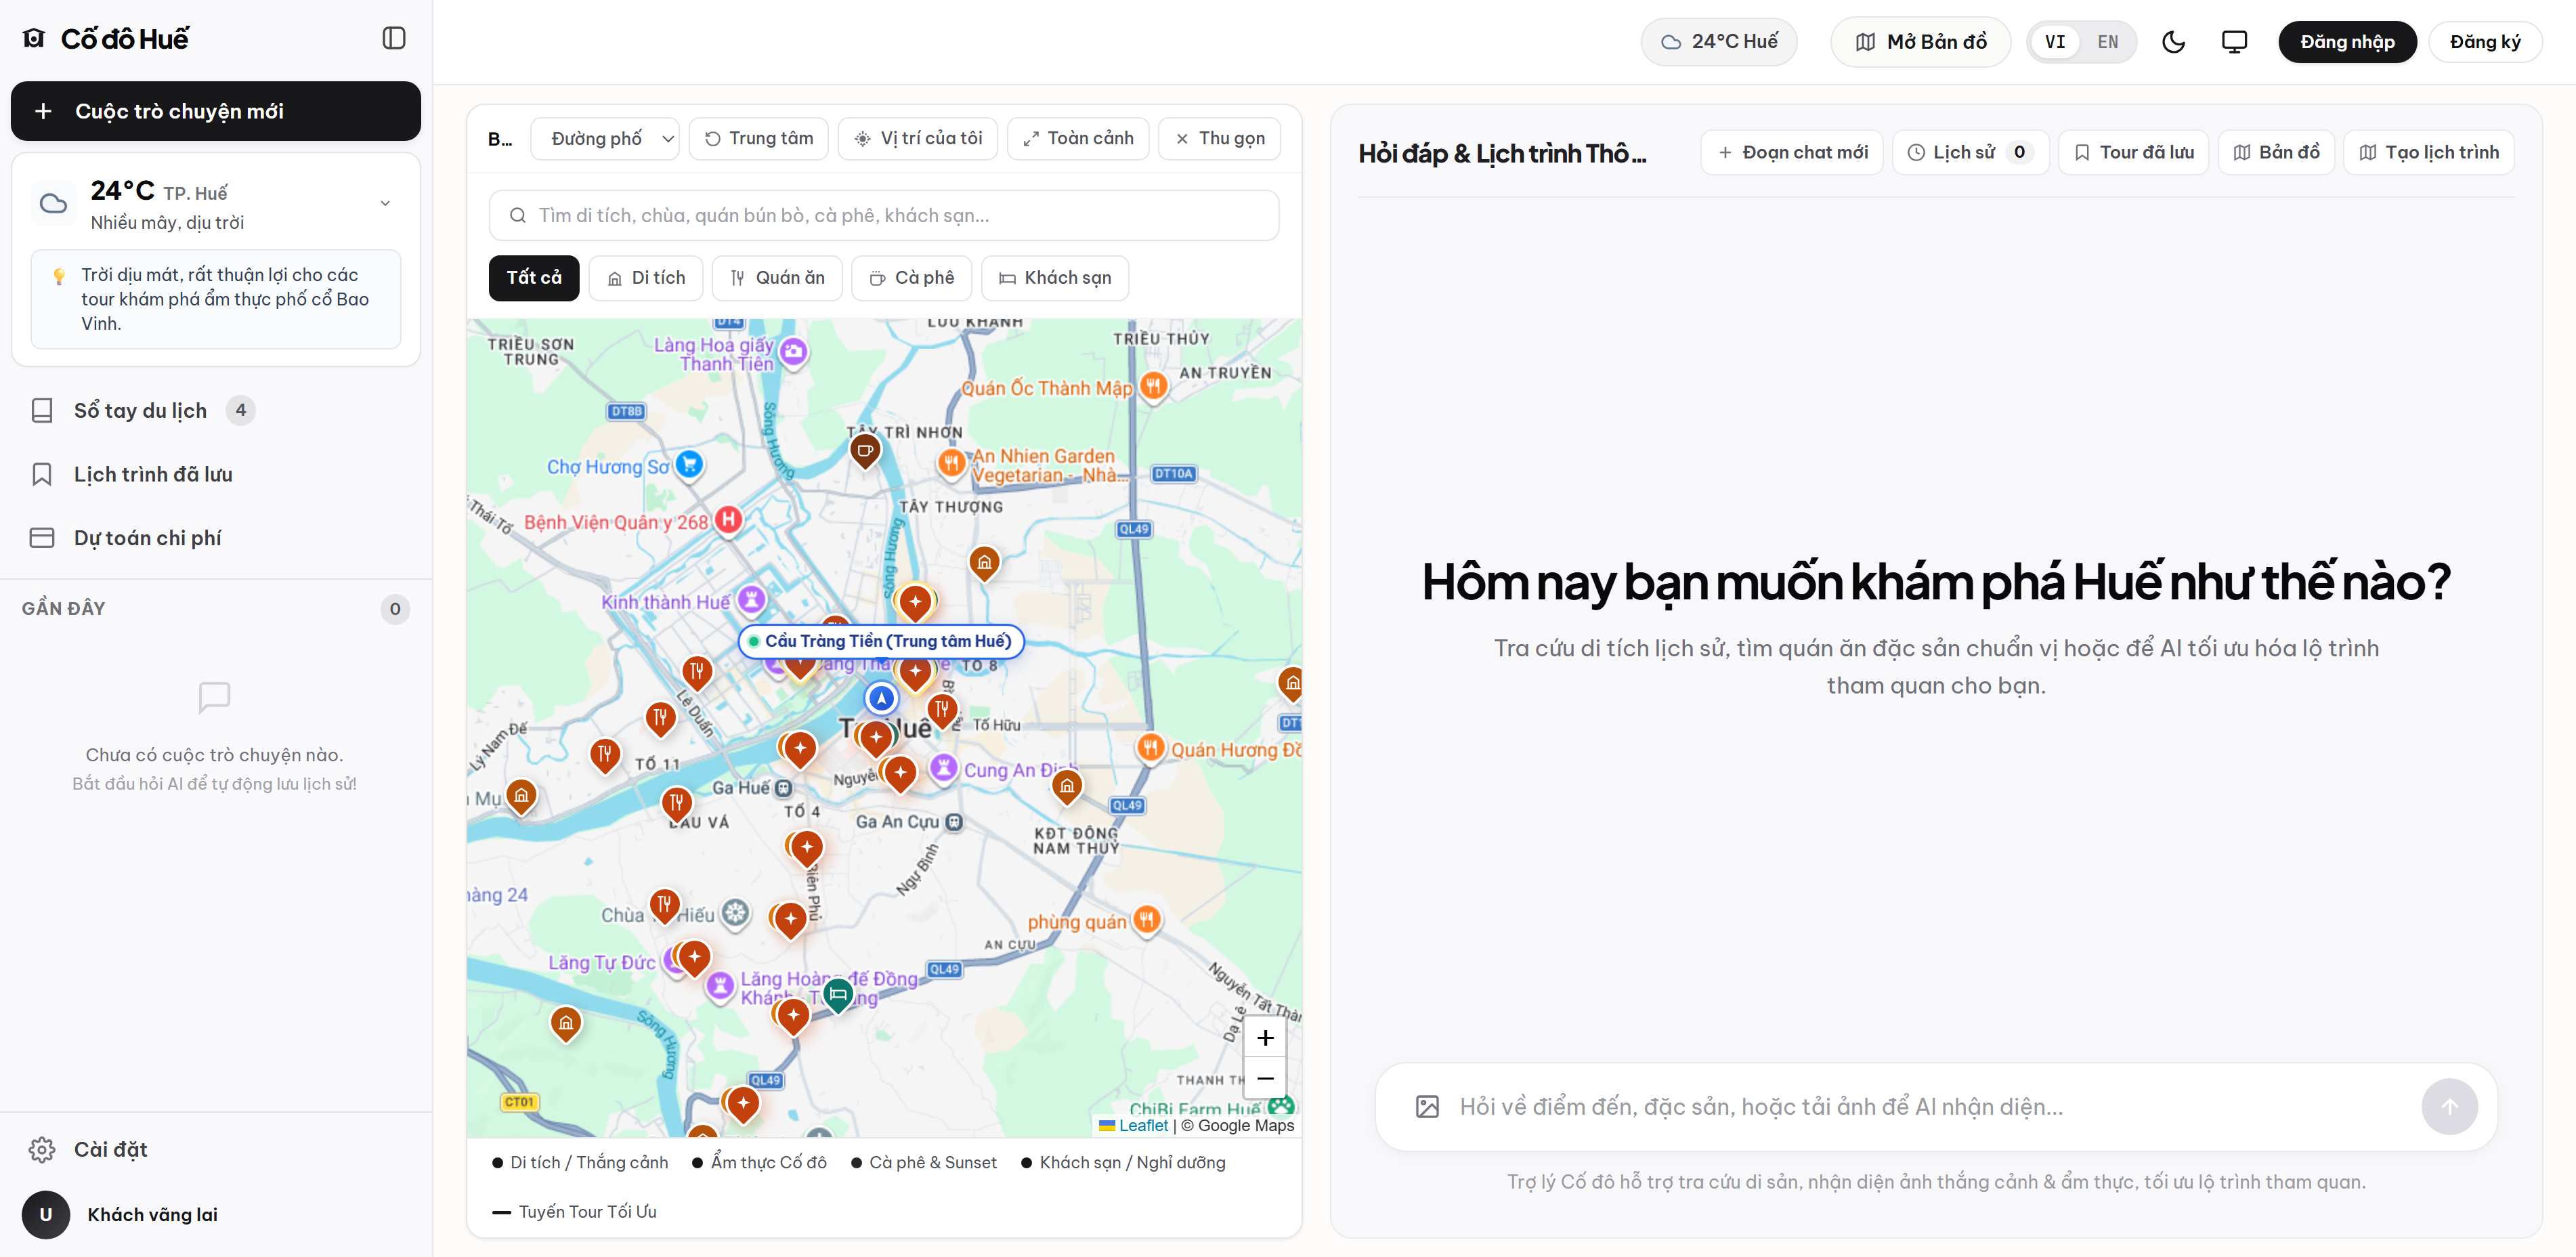
\includegraphics[width=0.98\textwidth]{img/web_main_interface.png}
    \caption{Giao diện chính toàn cảnh của Hệ thống Web Spatial GraphRAG Cố đô Huế}
    \label{fig:web_main_interface}
\end{figure}

\clearpage
\subsection*{C.2. Luồng Hỏi đáp Tác tử Spatial GraphRAG với Trích dẫn XAI và Thẻ Ghim Địa điểm}

Khi du khách đặt câu hỏi truy vấn không gian phức tạp (ví dụ: \textit{«Ăn bún bò ở đâu ngon và gần Đại Nội Huế nhất?»}), hệ thống kích hoạt luồng tác tử truy xuất đồ thị tri thức và hiển thị minh bạch toàn bộ chuỗi lập luận (Hình \ref{fig:web_chat_spatial_rag}):
\begin{itemize}
    \item \textbf{Chuỗi lập luận có thể giải thích (Explainable Graph Trace - XAI):} Trình bày trực quan tiến trình xử lý gồm 4 bước: (1) Phân loại ý định ẩm thực; (2) Lọc bán kính không gian ($d \le 1{,}5\text{ km}$); (3) Khai thác liên kết quan hệ trong Đồ thị Tri thức NetworkX; và (4) Đánh giá điểm tin cậy ngữ cảnh với thước đo đồ họa trực quan (đạt $94\%$, vượt ngưỡng kiểm soát nội bộ $0{,}40$ để sinh câu trả lời từ tri thức đồ thị).
    \item \textbf{Thẻ địa điểm gợi ý tương tác (POI Action Cards):} Cung cấp các nút tương tác gắn biểu tượng chuyên biệt (Bún bò Mụ Rơi, Đại Nội Huế, Chợ Đông Ba) cho phép ghim trực tiếp tọa độ lên bản đồ GIS chỉ với một thao tác nhấp chuột.
\end{itemize}

\begin{figure}[H]
    \centering
    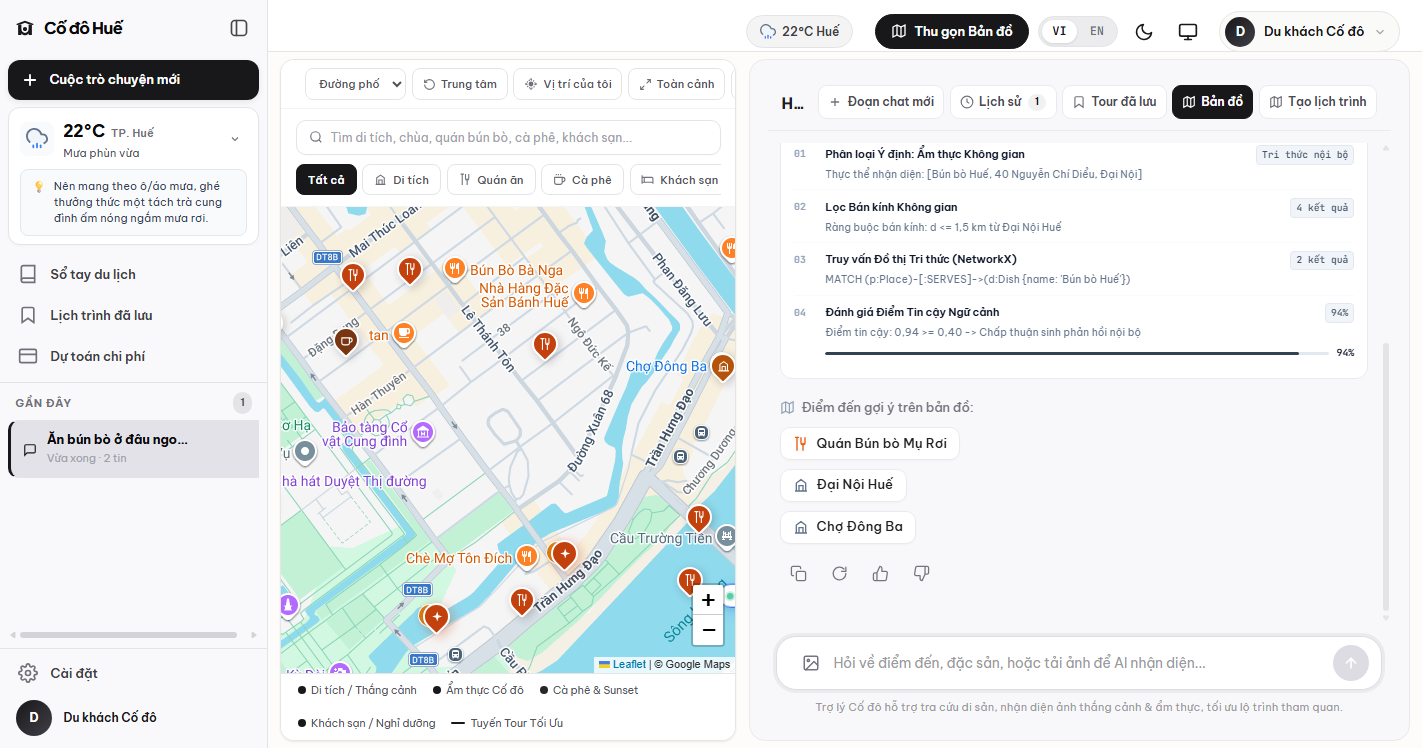
\includegraphics[width=0.98\textwidth]{img/web_chat_spatial_rag.png}
    \caption{Phản hồi trực quan của Trợ lý AI kết hợp Cây suy luận XAI và Thẻ tương tác Địa điểm}
    \label{fig:web_chat_spatial_rag}
\end{figure}

\clearpage
\subsection*{C.3. Trực quan hóa Tuyến Tour Tối ưu và Điều hướng Chặng OSRM trên Bản đồ GIS}

Để phục vụ bài toán di chuyển thực tế của du khách, hệ thống tích hợp công cụ mô phỏng đường đi chính xác theo mạng lưới giao thông đô thị Huế (Hình \ref{fig:web_route_itinerary_map}):
\begin{itemize}
    \item \textbf{Đường đa giác tuyến đường (OSRM Tour Route Polyline):} Vẽ tuyến đường liên kết thông suốt từ điểm xuất phát (Cầu Tràng Tiền) qua các điểm di tích và ẩm thực (Đại Nội $\to$ Bún bò Mụ Rơi $\to$ Chùa Thiên Mụ $\to$ Lăng Tự Đức) bám sát các cây cầu và cung đường ven sông Hương.
    \item \textbf{Bộ đánh số chặng dừng chân:} Đánh số thứ tự trực quan từng điểm đến ($A, 2, 3, 4$), hỗ trợ du khách hình dung rõ ràng thứ tự hành trình theo thứ tự không gian tối ưu.
\end{itemize}

\begin{figure}[H]
    \centering
    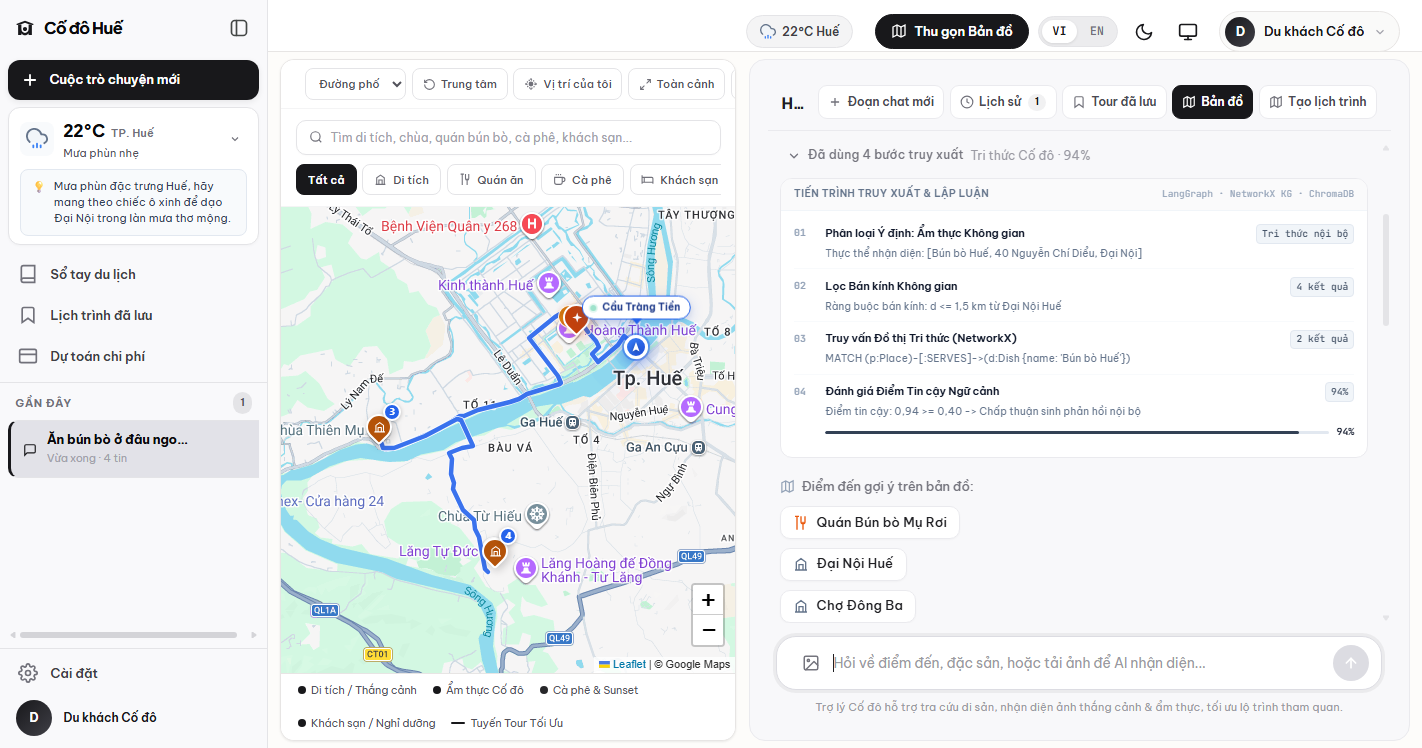
\includegraphics[width=0.98\textwidth]{img/web_route_itinerary_map.png}
    \caption{Lộ trình tham quan thực tế theo mạng lưới giao thông đường bộ Cố đô Huế}
    \label{fig:web_route_itinerary_map}
\end{figure}

\clearpage
\subsection*{C.4. Công cụ Khởi tạo Nhanh Lịch trình theo Điểm Xuất phát GPS và Khẩu vị}

Nhằm nâng cao trải nghiệm người dùng, hệ thống cung cấp thẻ lập lịch trình nhanh ngay trên giao diện bản đồ (Hình \ref{fig:web_quick_planner}):
\begin{itemize}
    \item \textbf{Tự động định vị điểm xuất phát:} Nhận diện tọa độ GPS thực tế của du khách hoặc mặc định tại điểm trung tâm Cố đô (Cầu Tràng Tiền).
    \item \textbf{Tùy biến tham số hành trình:} Cho phép lựa chọn thời lượng chuyến đi (1, 2, 3 ngày), nhóm đối tượng đồng hành (Cặp đôi, Gia đình, Bạn bè) và danh mục các món ăn đặc sản ưu tiên thưởng thức thông qua hệ thống nút chọn nhanh (\textit{Tag Pills}).
\end{itemize}

\begin{figure}[H]
    \centering
    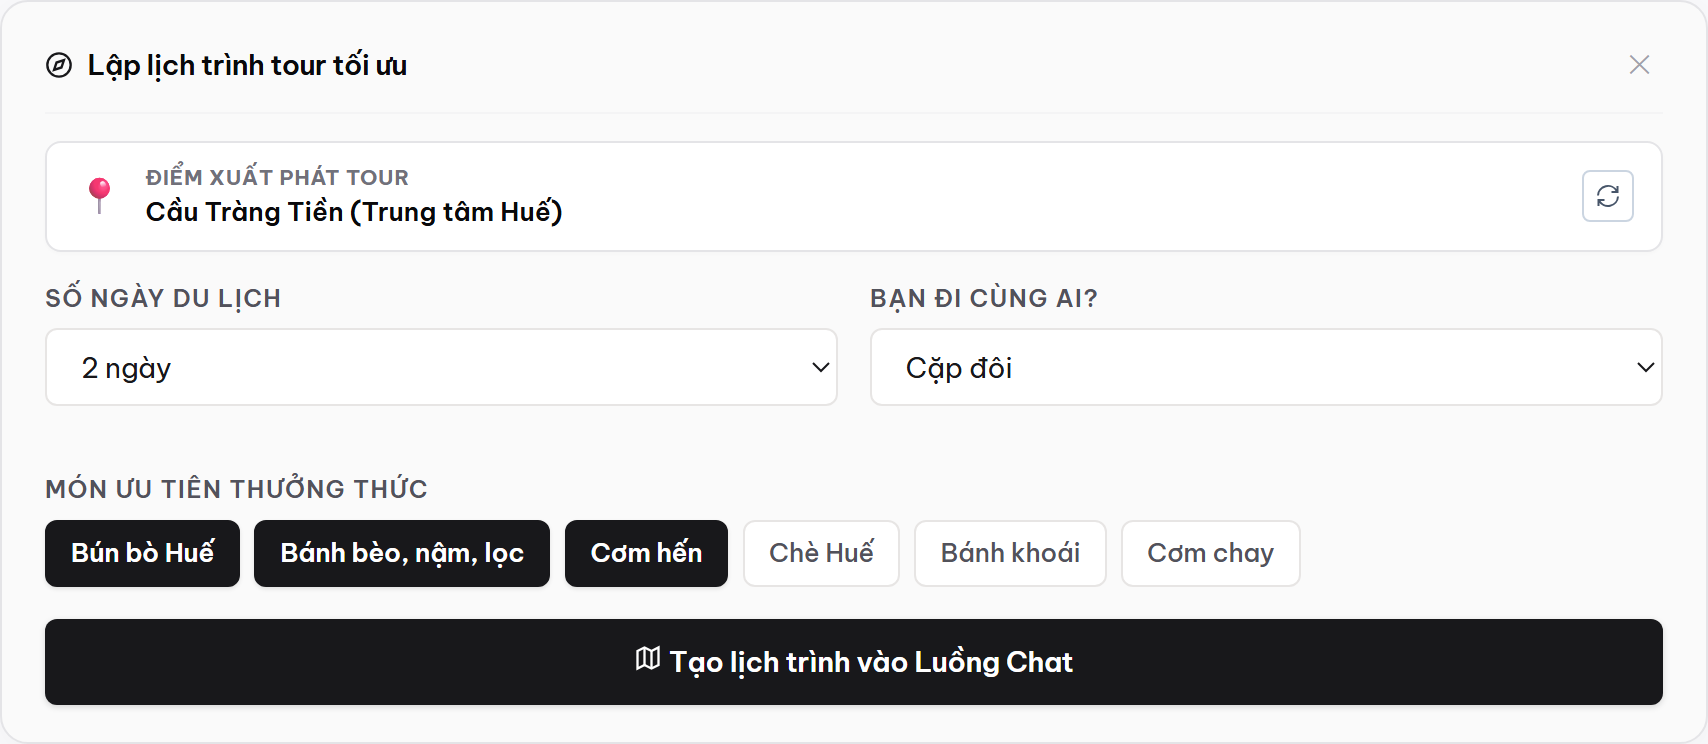
\includegraphics[width=0.92\textwidth]{img/web_quick_planner.png}
    \caption{Thẻ công cụ tạo nhanh tour du lịch theo vị trí xuất phát GPS và khẩu vị ẩm thực}
    \label{fig:web_quick_planner}
\end{figure}

\clearpage
\subsection*{C.5. Tính năng Nhận diện Thị giác Di sản và Món ăn Đa phương thức (Multimodal Vision)}

Khung nhập liệu hội thoại hỗ trợ cơ chế tiếp nhận hình ảnh đa phương thức (Hình \ref{fig:web_multimodal_vision}):
\begin{itemize}
    \item \textbf{Thanh xem trước hình ảnh đính kèm (Image Preview Bar):} Cho phép du khách tải lên hình ảnh di tích kiến trúc hoặc món ăn thực tế chụp tại hiện trường.
    \item \textbf{Truy vấn kết hợp Đa phương thức:} Mô hình thị giác máy tính trích xuất đặc trưng hình ảnh, đối sánh với kho vector mẫu và Đồ thị Tri thức để định danh chính xác công trình di sản (Cổng Ngọ Môn) cùng thông tin lịch sử và vị trí trên bản đồ.
\end{itemize}

\begin{figure}[H]
    \centering
    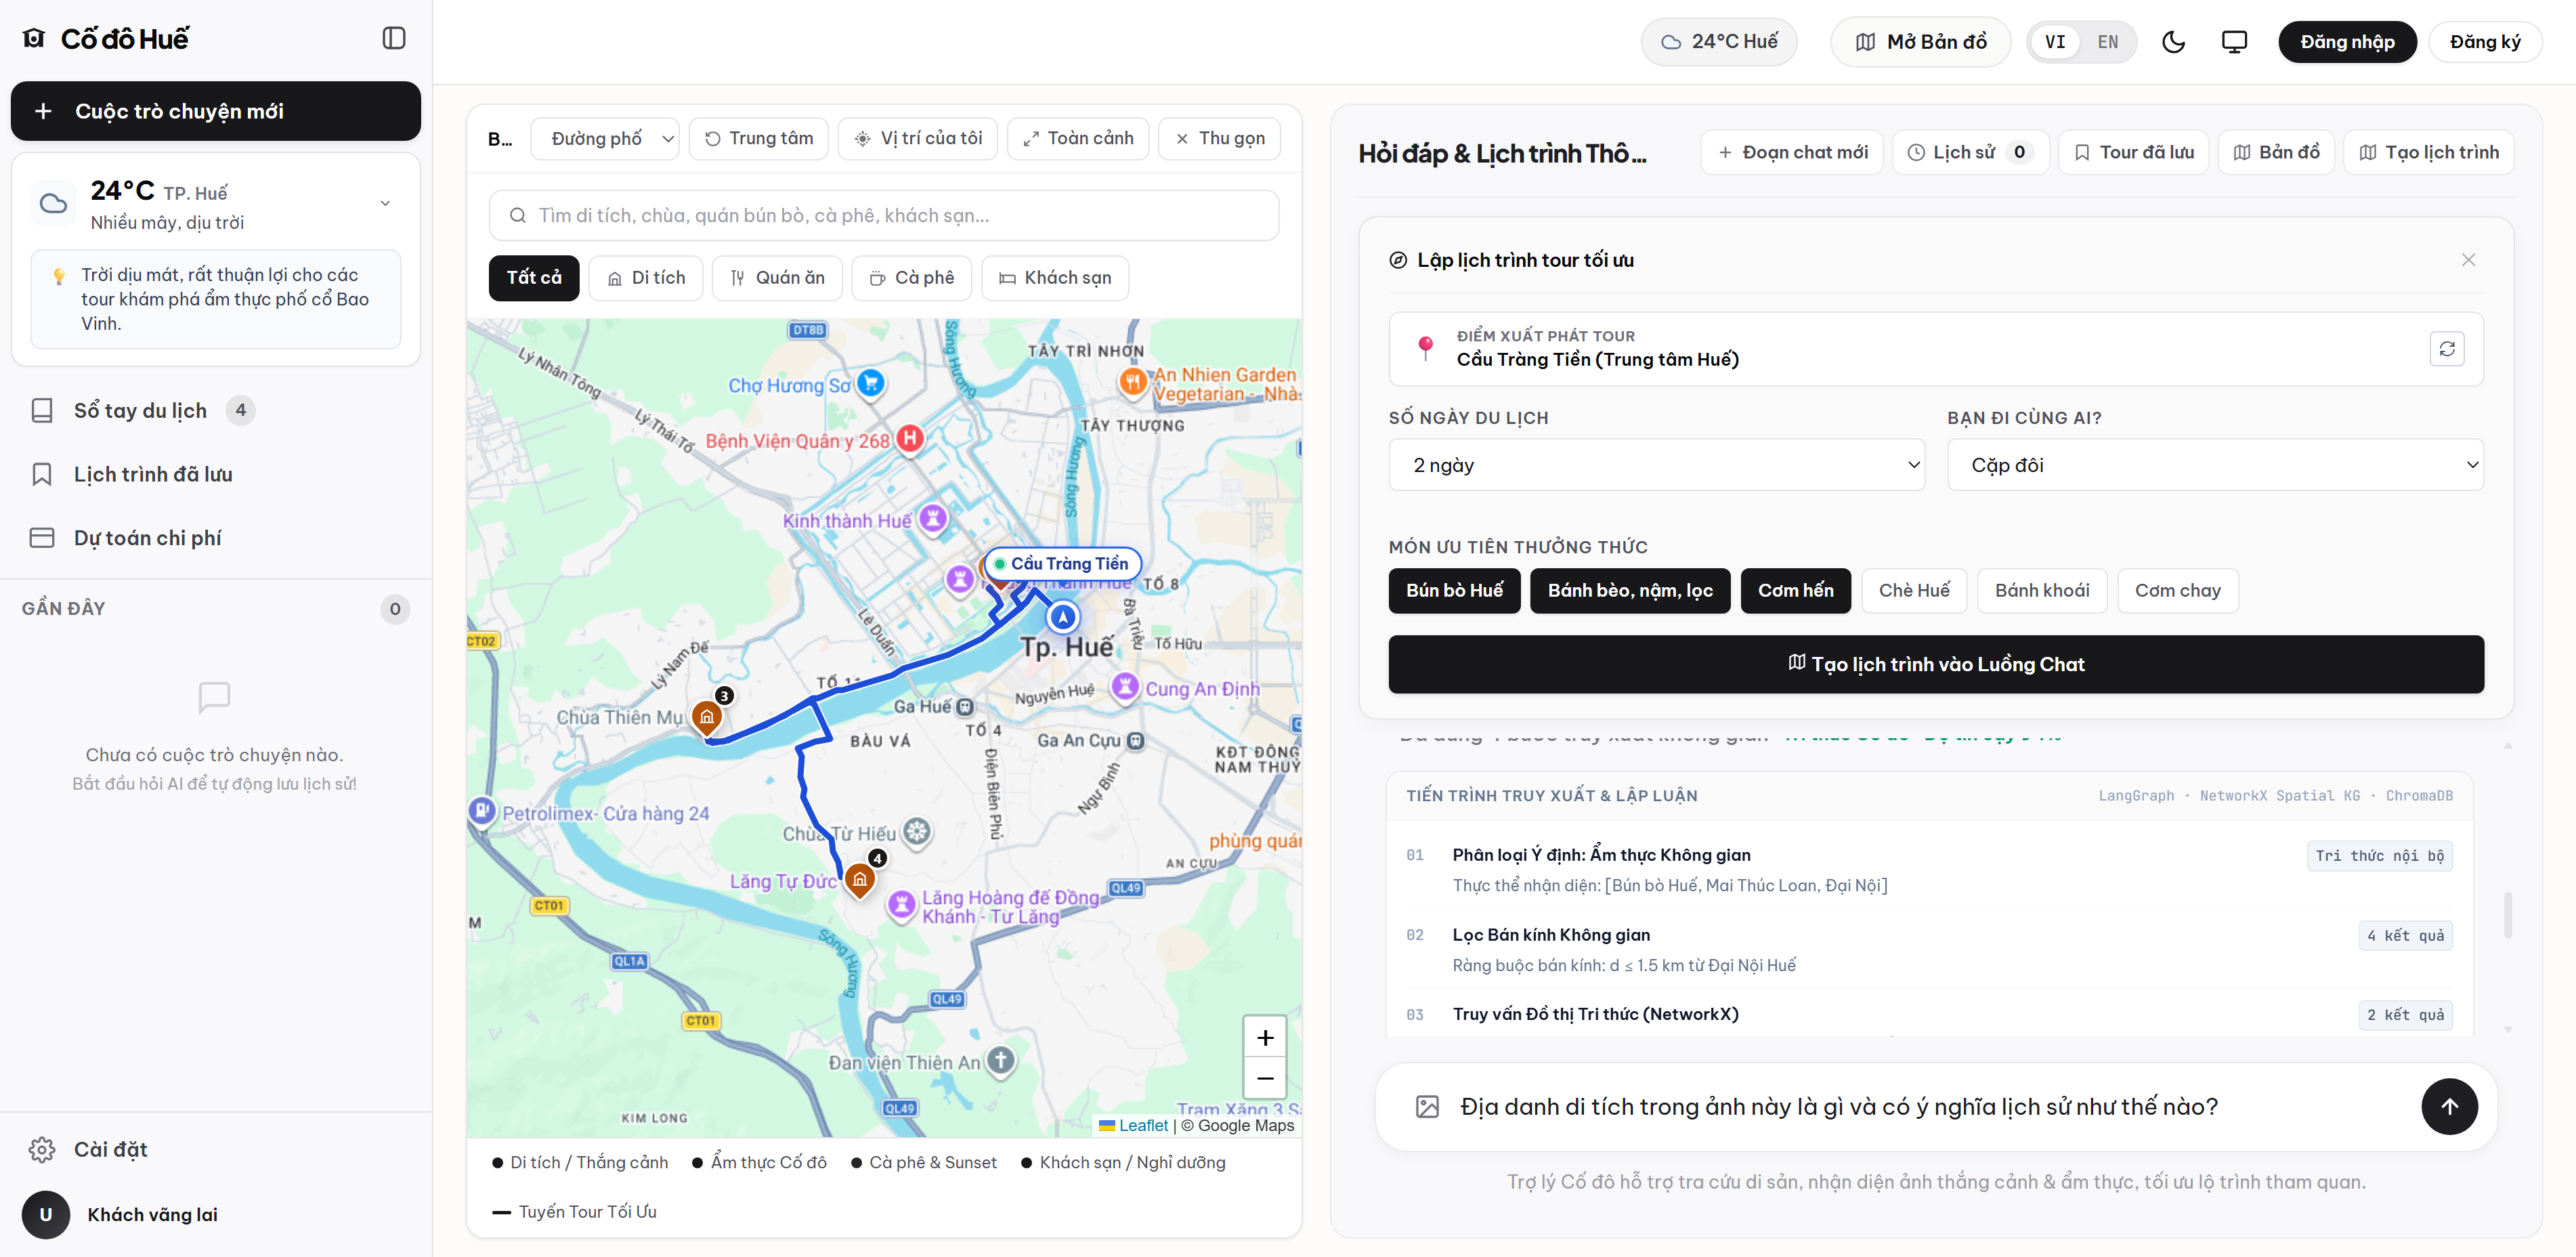
\includegraphics[width=0.98\textwidth]{img/web_multimodal_vision.png}
    \caption{Thanh tải ảnh và tính năng nhận diện thị giác di sản đa phương thức}
    \label{fig:web_multimodal_vision}
\end{figure}

\clearpage
\subsection*{C.6. Cửa sổ Cá nhân hóa Hồ sơ và Phong cách Du lịch (AI Traveler Persona Modal)}

Nhằm đáp ứng yêu cầu cá nhân hóa trong mô hình Spatial GraphRAG, hệ thống cung cấp giao diện quản lý hồ sơ du khách (Hình \ref{fig:web_traveler_persona}):
\begin{itemize}
    \item \textbf{Khẩu vị \& Dinh dưỡng đặc sản Huế:} Lựa chọn các cấp độ cay (Ăn cay chuẩn Huế, Ít cay/Vừa phải), thực đơn ăn chay (\textit{Vegetarian}), hoặc hạn chế dị ứng (Không ăn hải sản). Các tham số này được tác tử tự động nhúng vào cấu trúc truy vấn để lọc bỏ các cơ sở ăn uống không tương thích.
    \item \textbf{Phong cách trải nghiệm ưu tiên:} Tùy chọn trọng số trải nghiệm như \textit{Di sản \& Lịch sử}, \textit{Ẩm thực truyền thống}, \textit{Sống ảo \& Check-in}, hoặc \textit{Nghỉ dưỡng \& Thiên nhiên}.
    \item \textbf{Phương tiện di chuyển chính:} Lựa chọn phương tiện (Đi bộ/Xe đạp, Thuê xe máy, Taxi/Grab) để tác tử lập lịch trình tính toán vận tốc trung bình và ma trận khoảng cách OSRM phù hợp.
\end{itemize}

\begin{figure}[H]
    \centering
    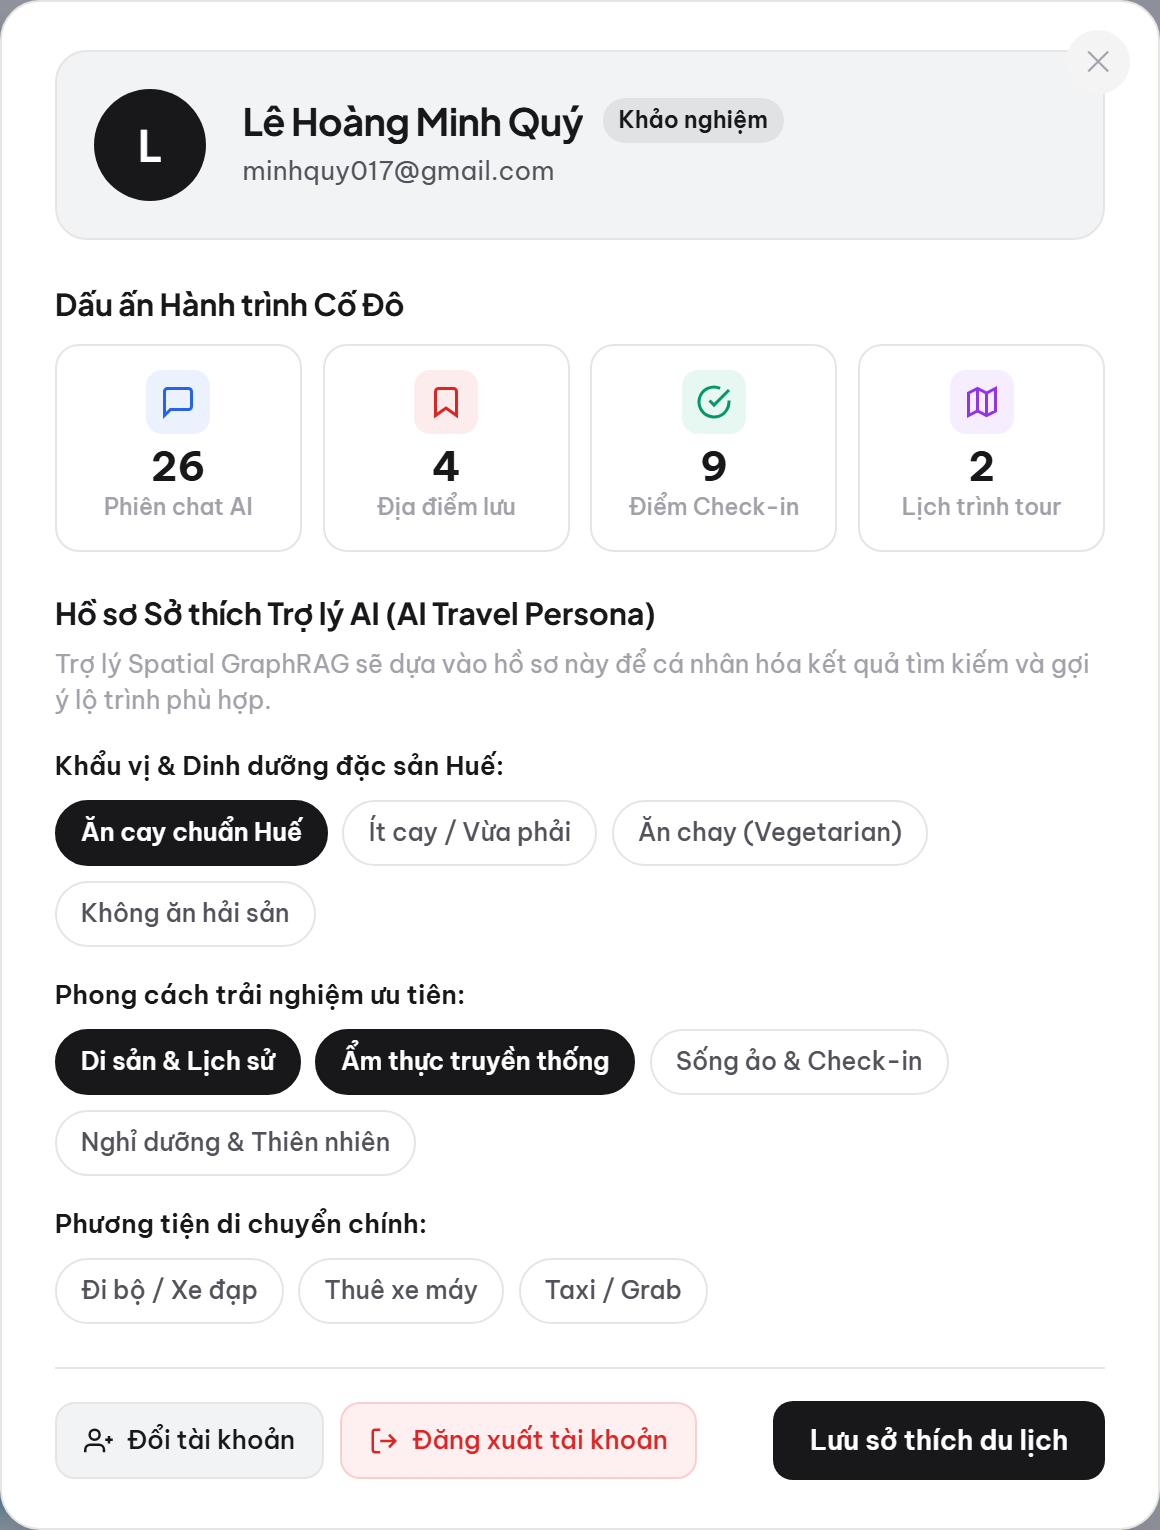
\includegraphics[width=0.56\textwidth]{img/web_traveler_persona.png}
    \caption{Cửa sổ Tùy biến Hồ sơ và Phong cách Du lịch của Du khách (AI Traveler Persona Modal)}
    \label{fig:web_traveler_persona}
\end{figure}

\clearpage
\subsection*{C.7. Giao diện Sổ tay Du lịch Cố Đô và Hộ chiếu Khám phá Di sản (Heritage Passport Modal)}

Giao diện Sổ tay du lịch Cố Đô (Hình \ref{fig:web_heritage_passport}) đóng vai trò lưu vết hành trình và thúc đẩy tương tác trải nghiệm văn hóa thông qua cơ chế trò chơi hóa (\textit{Gamification}):
\begin{itemize}
    \item \textbf{Hộ chiếu Khám phá (Discovery Passport):} Theo dõi tiến độ tham quan qua thanh cấp độ người dùng (\textit{Explorer Level Tag} từ Cấp 01 - \textit{Khách bộ hành Cố Đô} đến Cấp 04 - \textit{Chuyên gia Di sản Cố Đô}). Mỗi điểm di tích hoặc quán ăn du khách đặt chân đến được đánh dấu tem mộc check-in cùng mốc thời gian thực tế.
    \item \textbf{Danh mục Yêu thích (Wishlist):} Lưu trữ các địa điểm do du khách chủ động đánh dấu trên bản đồ để đưa vào kế hoạch tham quan tiếp theo.
\end{itemize}

\begin{figure}[H]
    \centering
    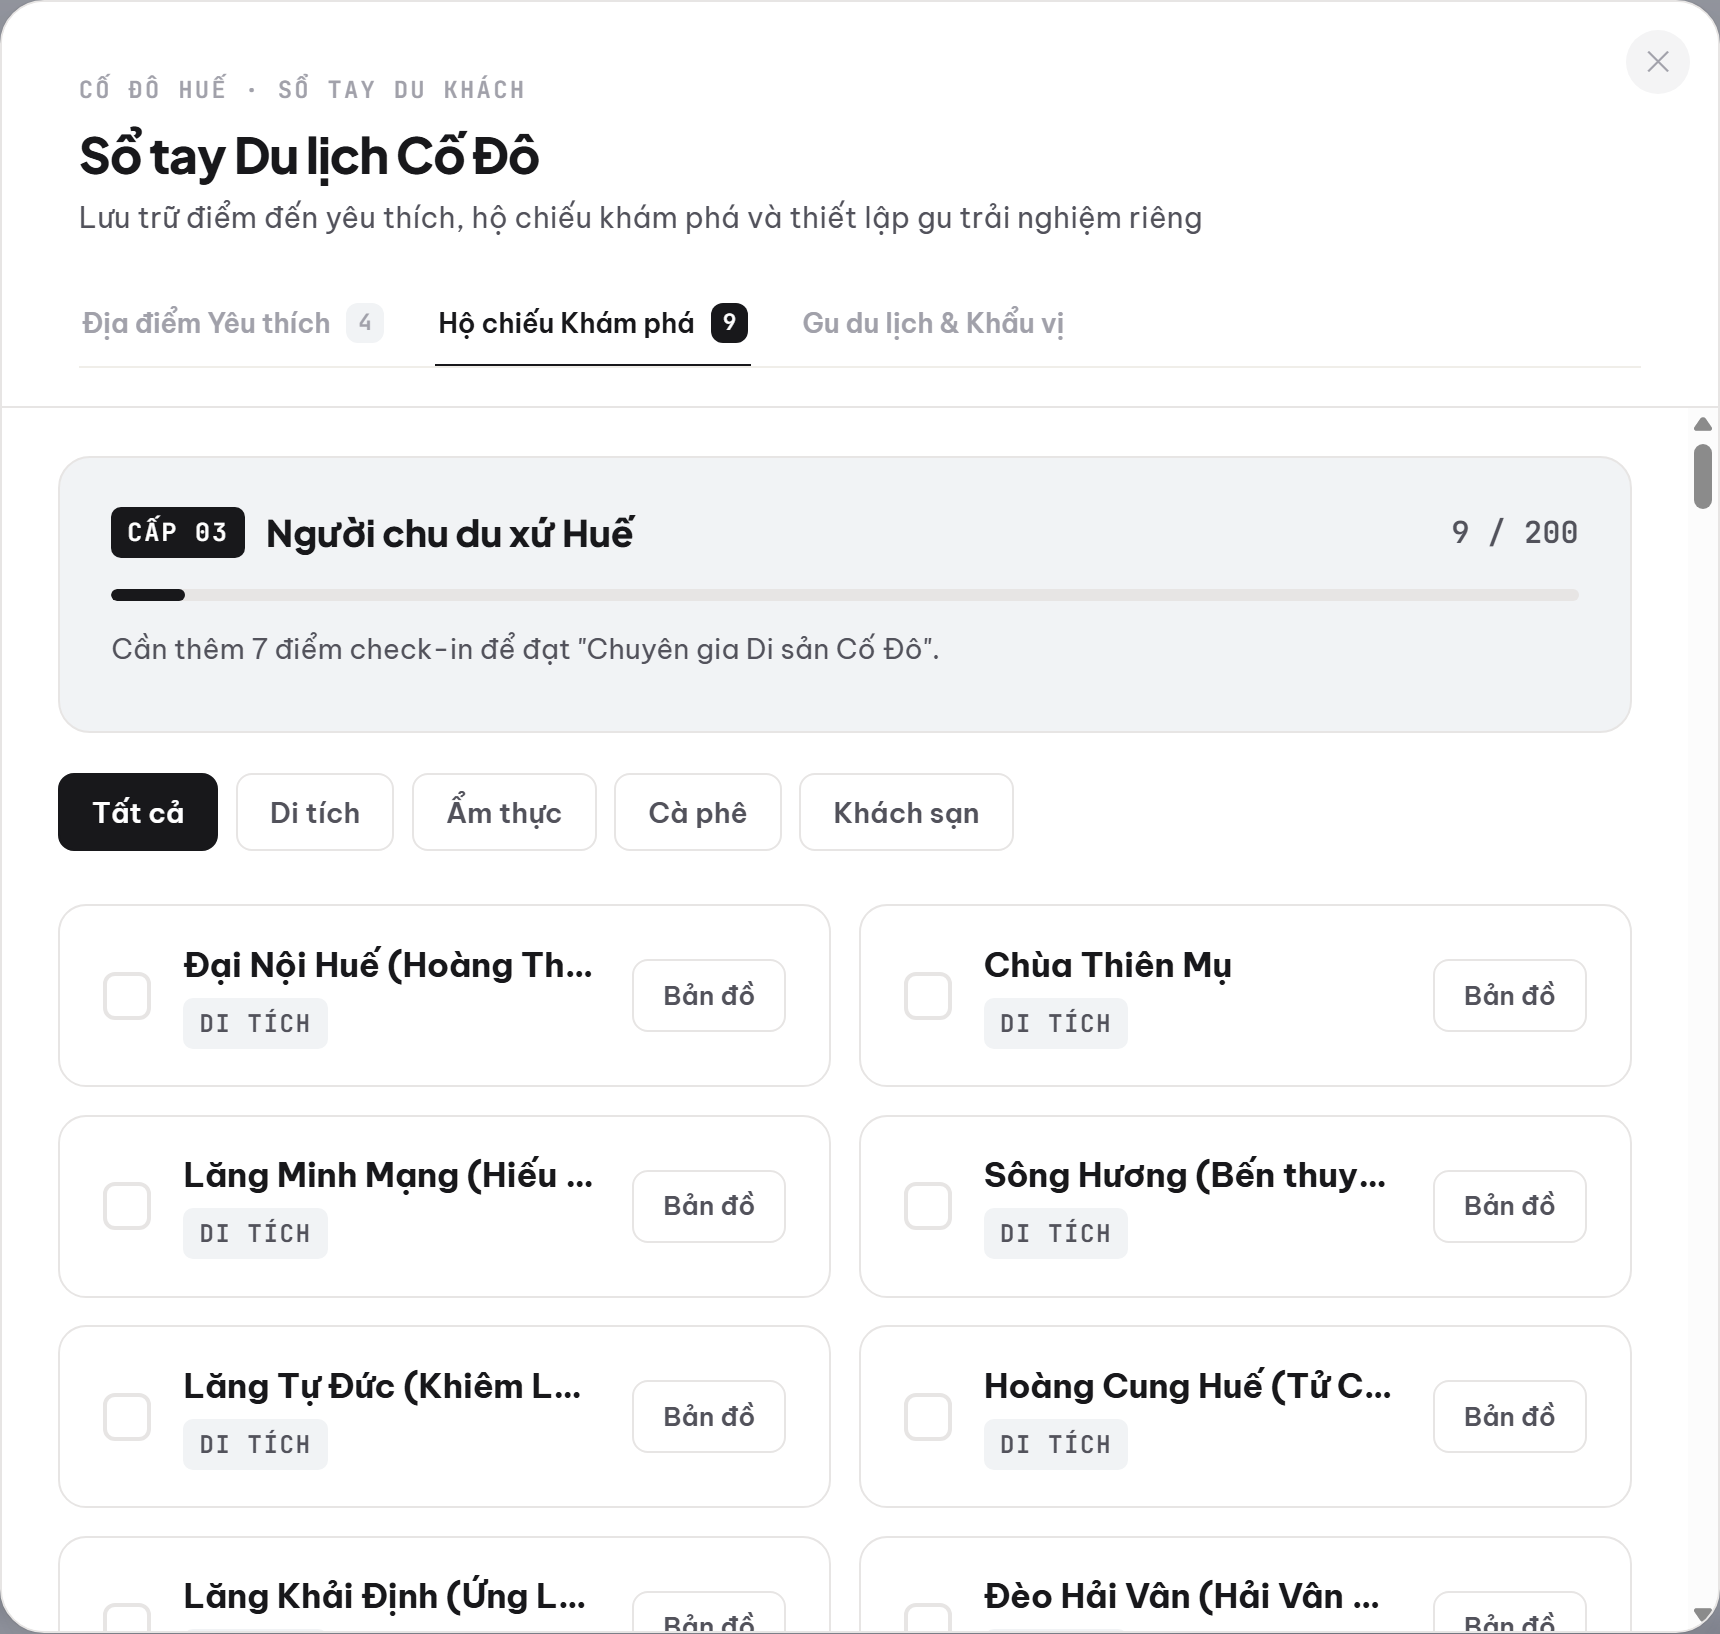
\includegraphics[width=0.80\textwidth]{img/web_heritage_passport.png}
    \caption{Giao diện Sổ tay Du lịch Cố Đô và Hộ chiếu Khám phá Di sản (Heritage Passport Modal)}
    \label{fig:web_heritage_passport}
\end{figure}

\clearpage
\subsection*{C.8. Bảng Dự toán Ngân sách Lịch trình Du lịch Chi tiết (Trip Budget Estimator Modal)}

Bảng dự toán ngân sách (Hình \ref{fig:web_trip_budget}) cung cấp công cụ tự động bóc tách chi phí minh bạch cho toàn bộ tour tham quan do tác tử AI khởi tạo:
\begin{itemize}
    \item \textbf{Biểu phí vé tham quan chính thức:} Tự động tra cứu giá vé niêm yết từ Trung tâm Bảo tồn Di tích Cố đô Huế (áp dụng chính sách miễn/giảm cho trẻ em và gói vé tuyến di tích gộp).
    \item \textbf{Định mức ẩm thực \& Lưu trú:} Ước tính chi phí ăn uống theo số lượng thành viên đoàn và phong cách ẩm thực đã chọn trong hồ sơ cá nhân.
    \item \textbf{Chi phí di chuyển OSRM:} Tính toán cước phí phương tiện dựa trên tổng quãng đường di chuyển thực tế mô phỏng qua mạng lưới giao thông đường bộ.
\end{itemize}

\begin{figure}[H]
    \centering
    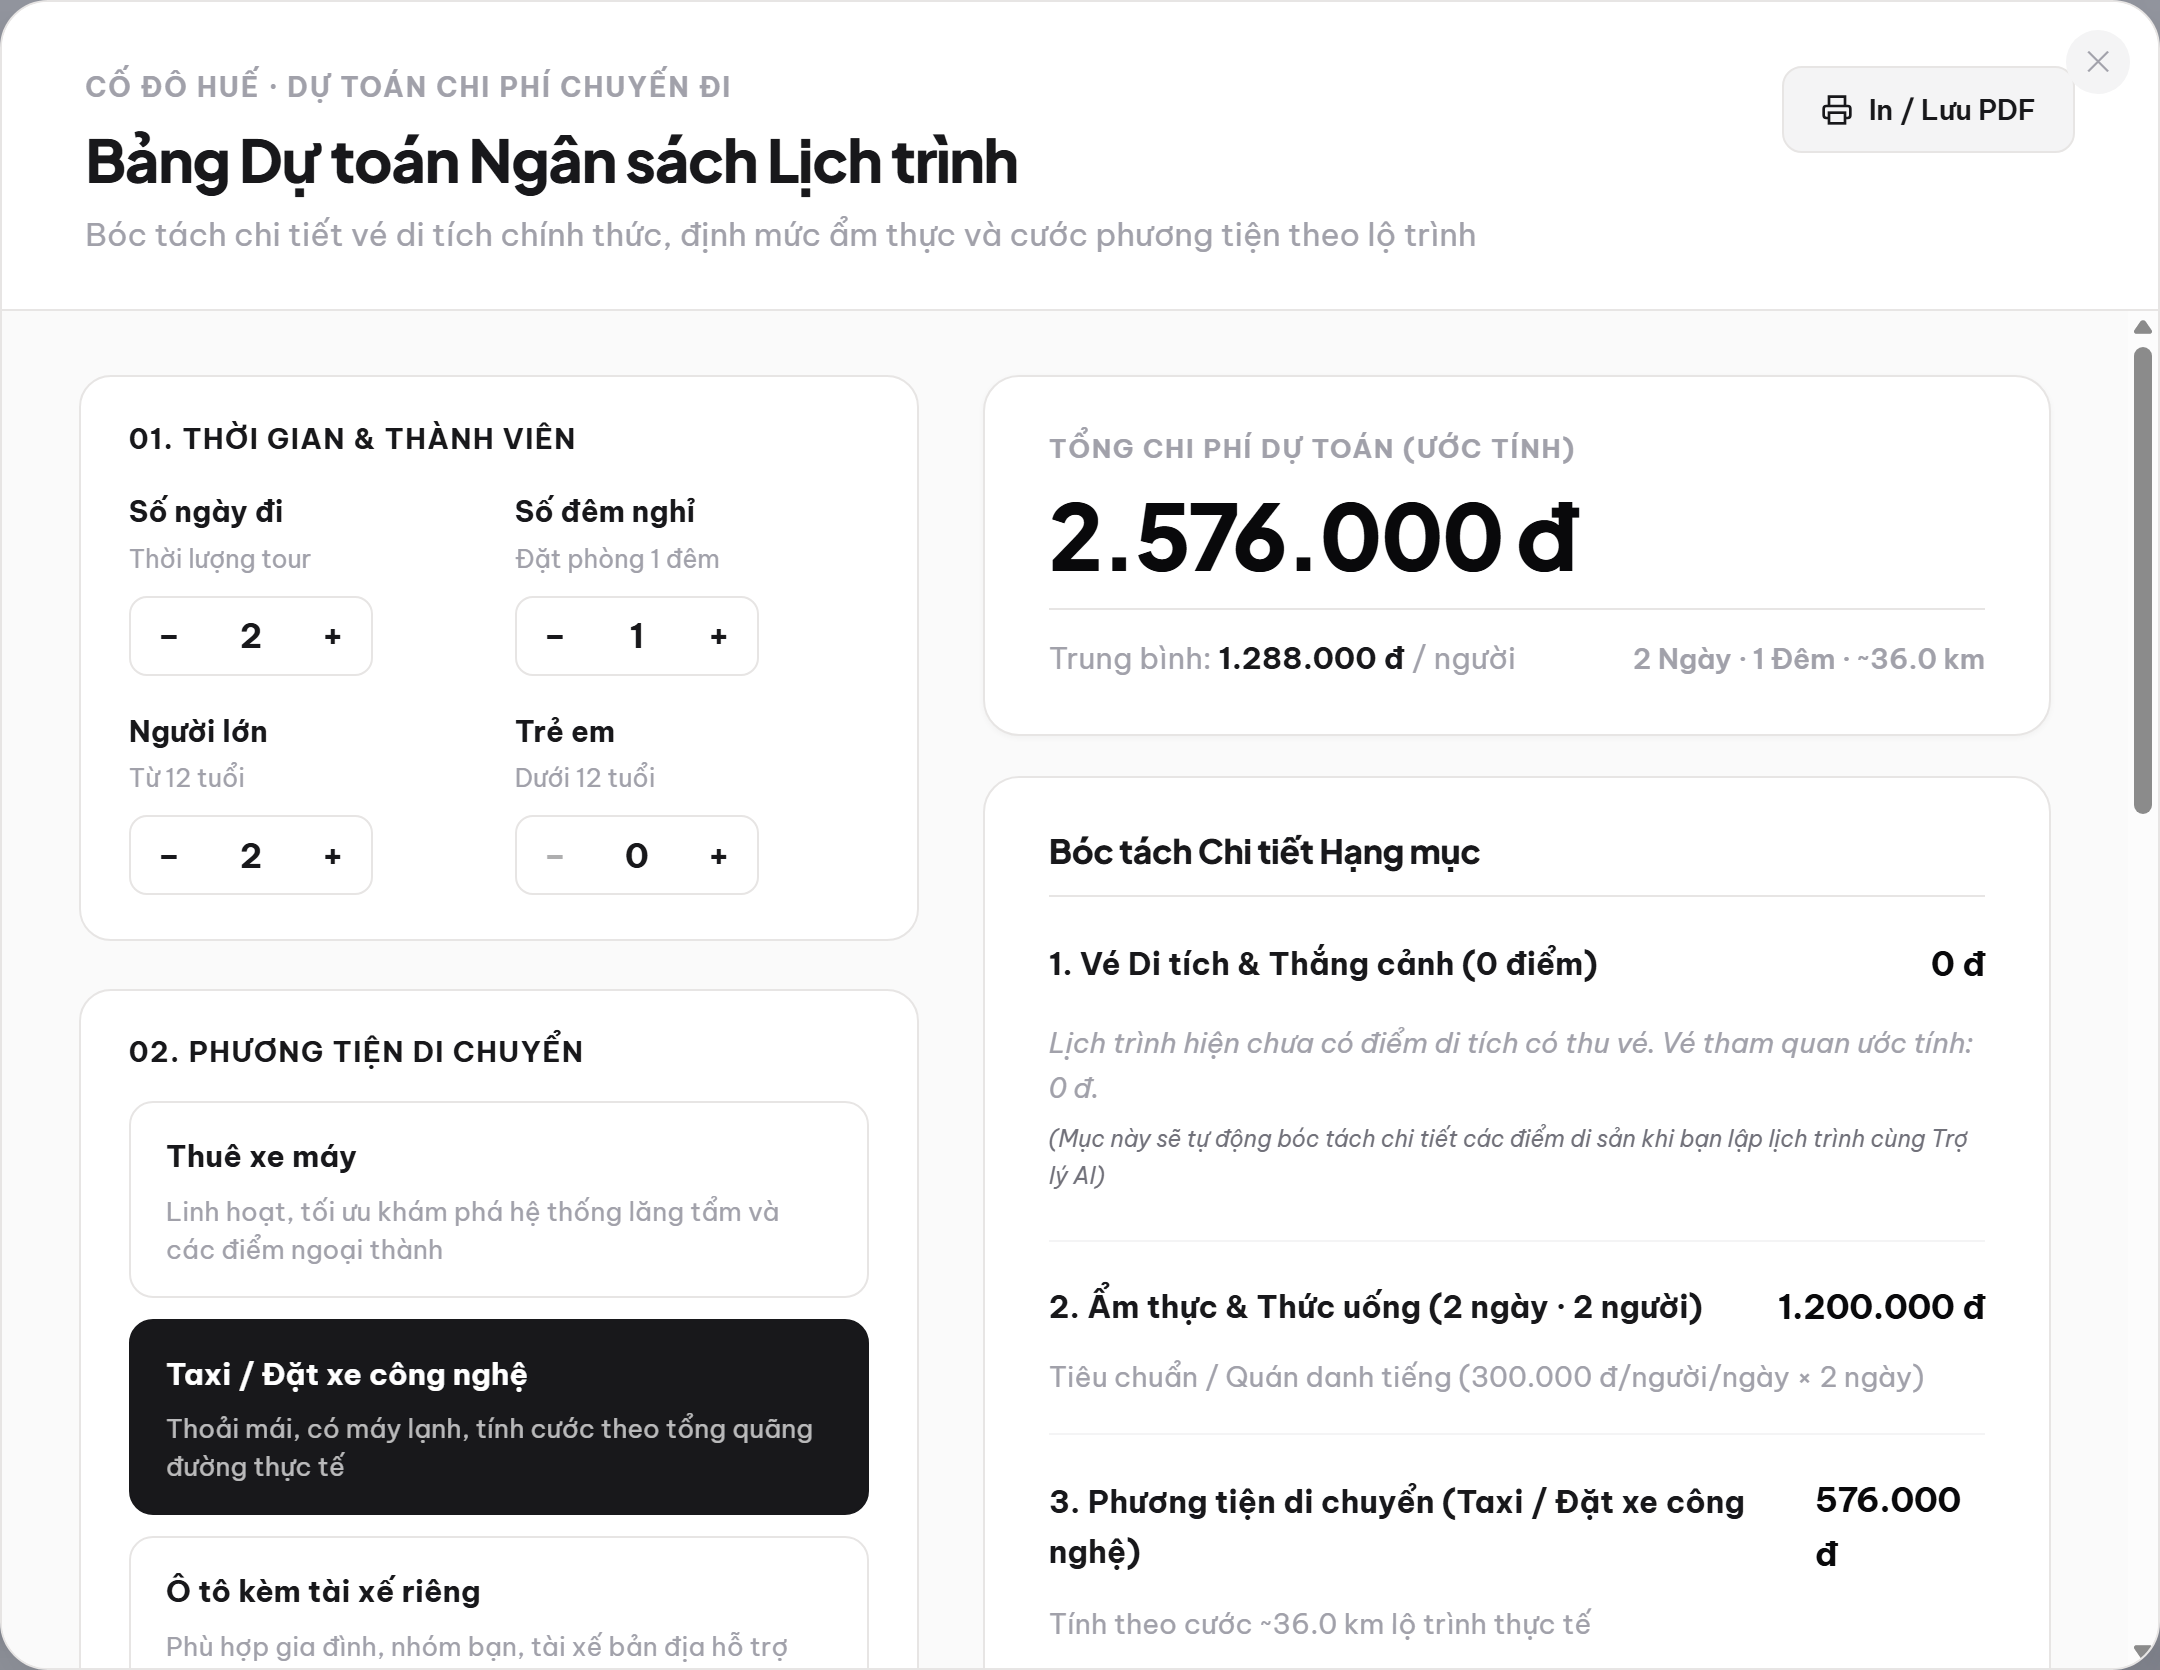
\includegraphics[width=0.88\textwidth]{img/web_trip_budget.png}
    \caption{Bảng Dự toán Ngân sách Lịch trình Du lịch Chi tiết (Trip Budget Estimator Modal)}
    \label{fig:web_trip_budget}
\end{figure}

\clearpage
\subsection*{C.9. Ngăn kéo Thông tin Chi tiết Địa điểm và Đánh giá Du khách (POI Details Drawer)}

Khi người dùng nhấn chọn bất kỳ biểu tượng địa danh nào trên bản đồ hoặc trong phản hồi của Trợ lý AI, hệ thống sẽ kích hoạt ngăn kéo trượt thông tin chuyên sâu (Hình \ref{fig:web_poi_details}):
\begin{itemize}
    \item \textbf{Hồ sơ văn hóa - lịch sử:} Trích xuất trực tiếp thuộc tính bản thể học từ Đồ thị Tri thức (tên chữ Hán, niên đại xây dựng, giá trị kiến trúc, địa chỉ hành chính, tọa độ GPS).
    \item \textbf{Đánh giá cộng đồng du khách:} Biểu đồ phân bổ sao đánh giá (từ 1 đến 5 sao), tỷ lệ đánh giá thực tế và khu vực viết nhận xét trải nghiệm có xác thực tài khoản.
    \item \textbf{Thanh tác vụ nhanh (Quick Actions):} Cung cấp các nút tương tác tức thì bao gồm: \textit{Yêu thích}, \textit{Check-in}, \textit{Mở Google Maps}, \textit{Chỉ đường từ vị trí hiện tại}, \textit{Thêm vào Tour} và \textit{Hỏi AI chi tiết về địa điểm này}.
\end{itemize}

\begin{figure}[H]
    \centering
    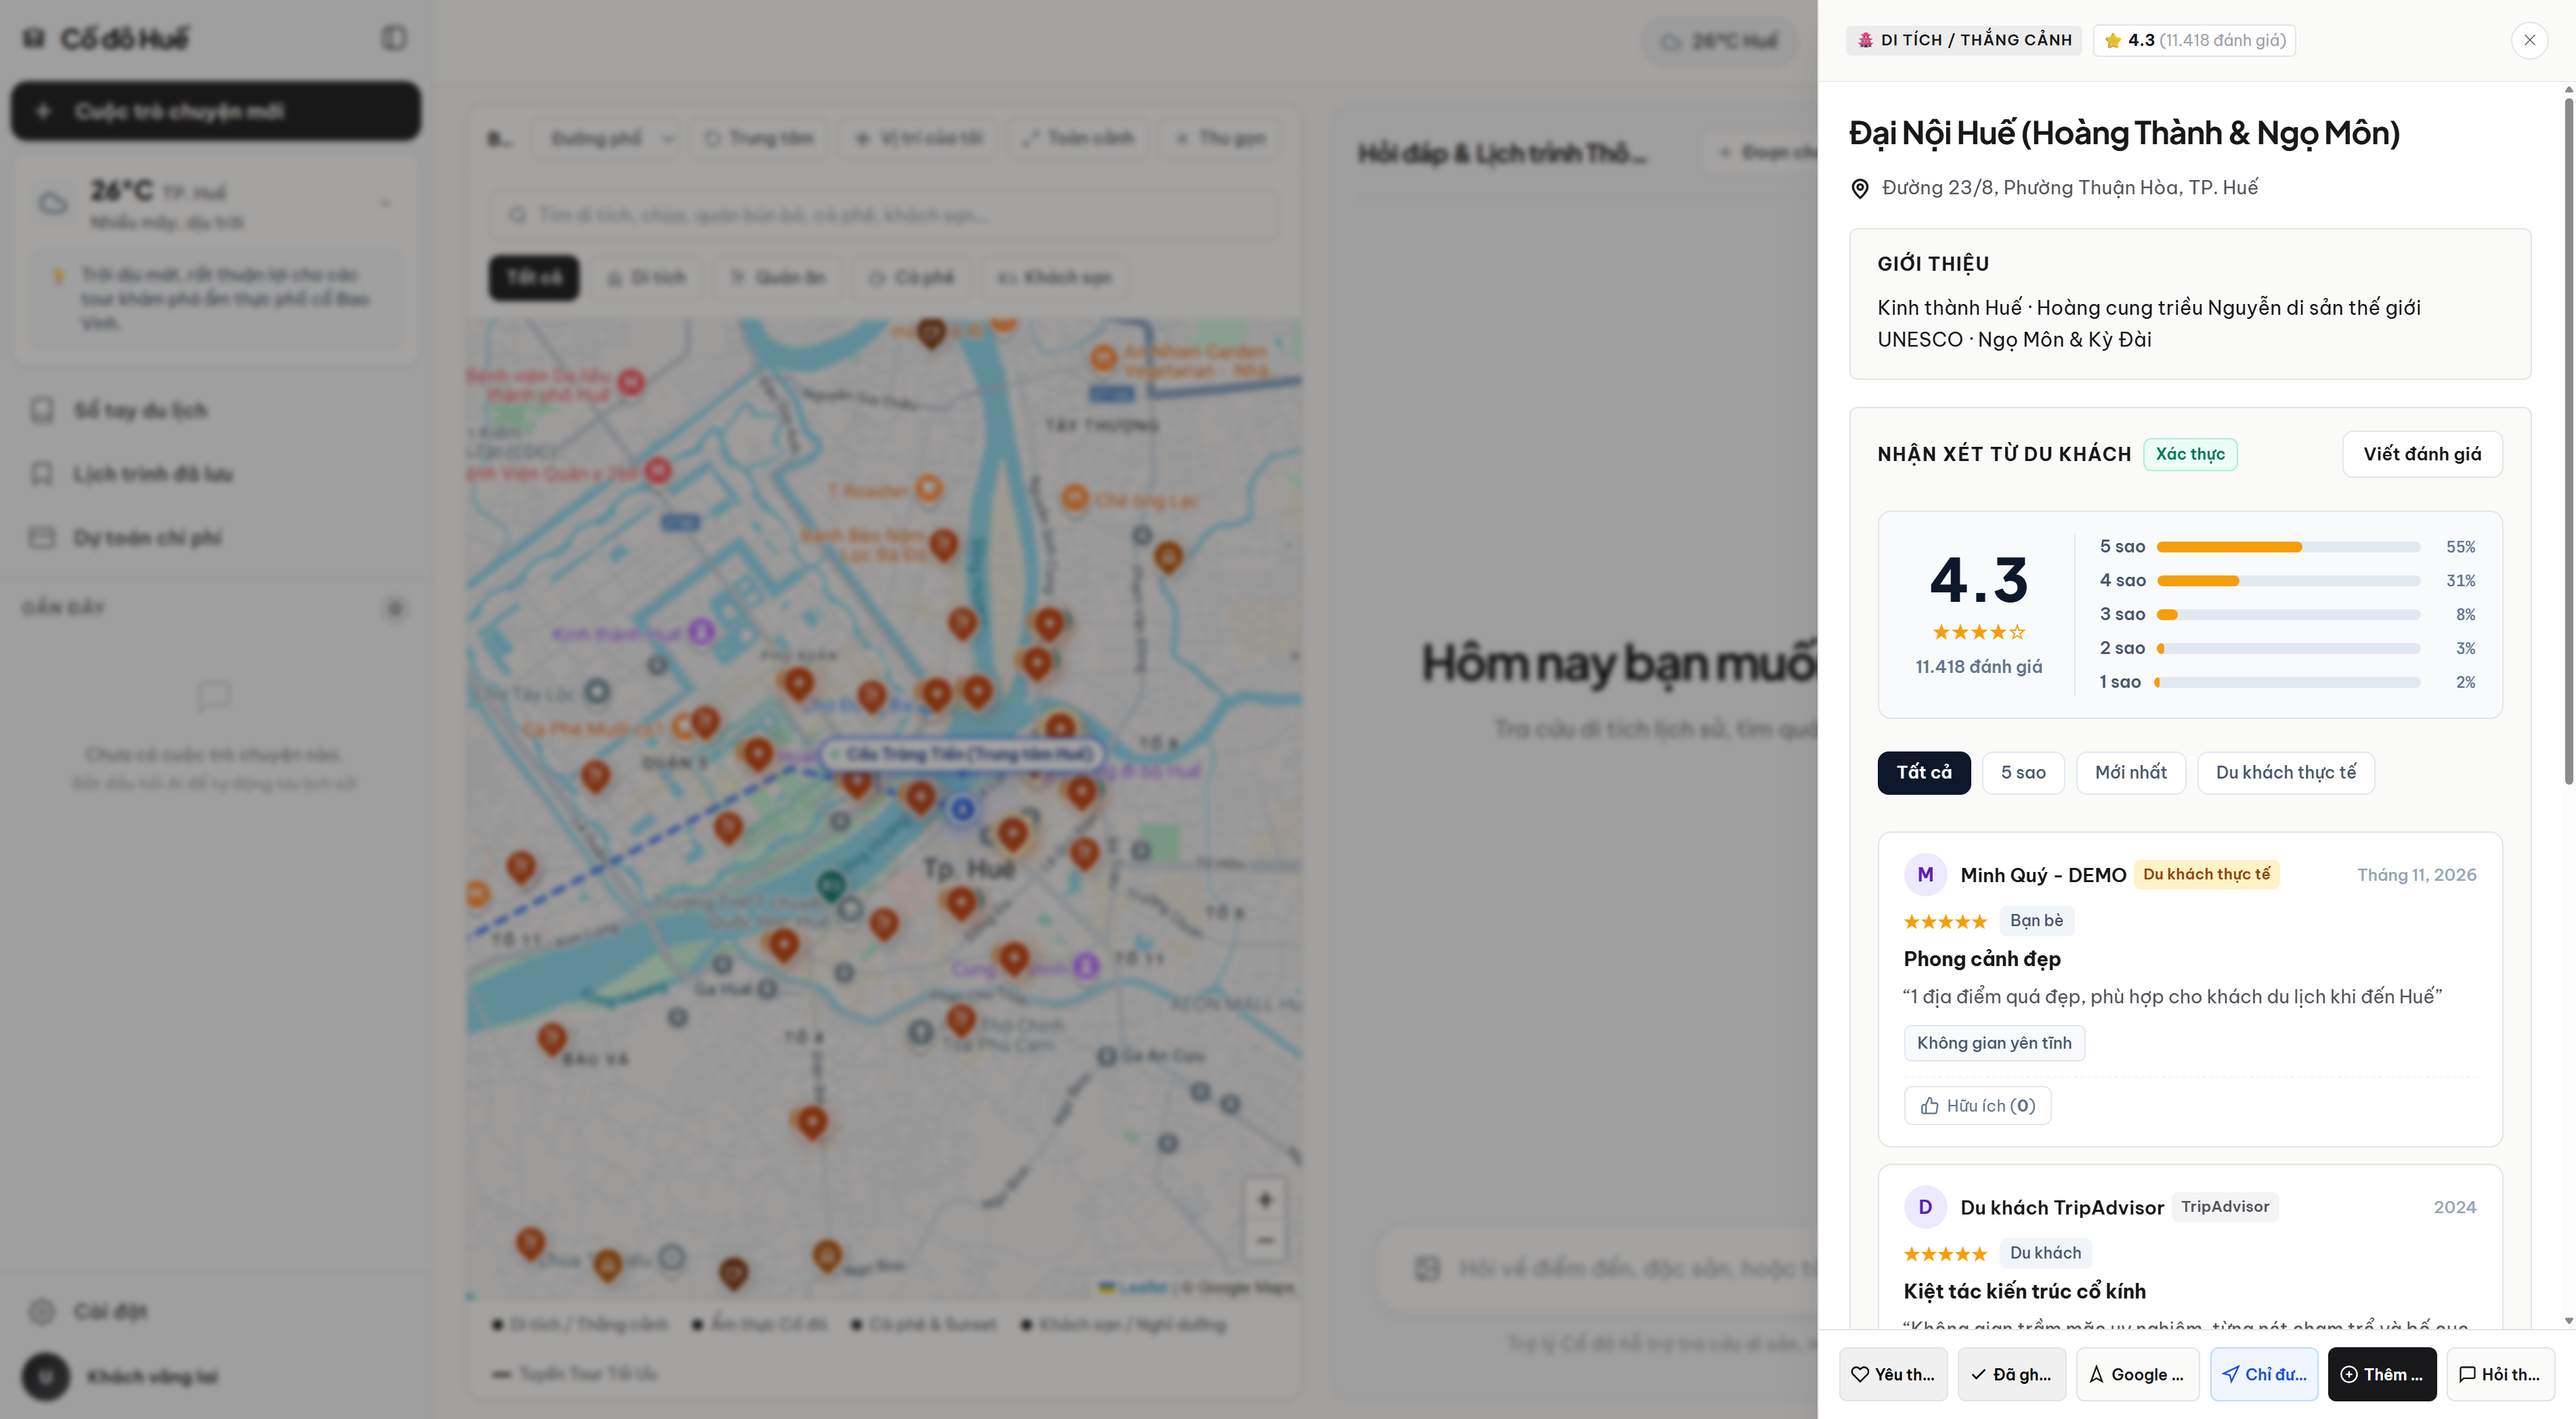
\includegraphics[width=0.98\textwidth]{img/web_poi_details.png}
    \caption{Ngăn kéo Thông tin Chi tiết Địa điểm và Đánh giá Du khách (POI Details Drawer)}
    \label{fig:web_poi_details}
\end{figure}

\clearpage
\subsection*{C.10. Cửa sổ Đóng góp Đánh giá và Phản hồi Trải nghiệm Du khách (POI Review Modal)}

Nhằm xây dựng kho dữ liệu phản hồi thực địa liên tục làm giàu cho hệ thống, ứng dụng cung cấp giao diện gửi đánh giá đa chiều (Hình \ref{fig:web_poi_review_modal}):
\begin{itemize}
    \item \textbf{Widget Chấm sao Tương tác:} Cho phép du khách đánh giá chất lượng từ 1 đến 5 sao kèm nhãn đánh giá tương ứng (\textit{5/5 · Tuyệt vời / Rất khuyến nghị}).
    \item \textbf{Thẻ phân loại mục đích \& Ấn tượng nổi bật:} Hệ thống các nút chọn nhanh phân loại mục đích chuyến đi (\textit{Gia đình, Cặp đôi, Bạn bè, Độc hành}) và các điểm ấn tượng (\textit{Cảnh quan đẹp, Không gian yên tĩnh, Kiến trúc độc đáo, Giá cả hợp lý}).
    \item \textbf{Khu vực nhận xét chi tiết:} Ô nhập nội dung chia sẻ cảm nhận thực tế với bộ đếm ký tự thời gian thực phục vụ tinh chỉnh dữ liệu đánh giá.
\end{itemize}

\begin{figure}[H]
    \centering
    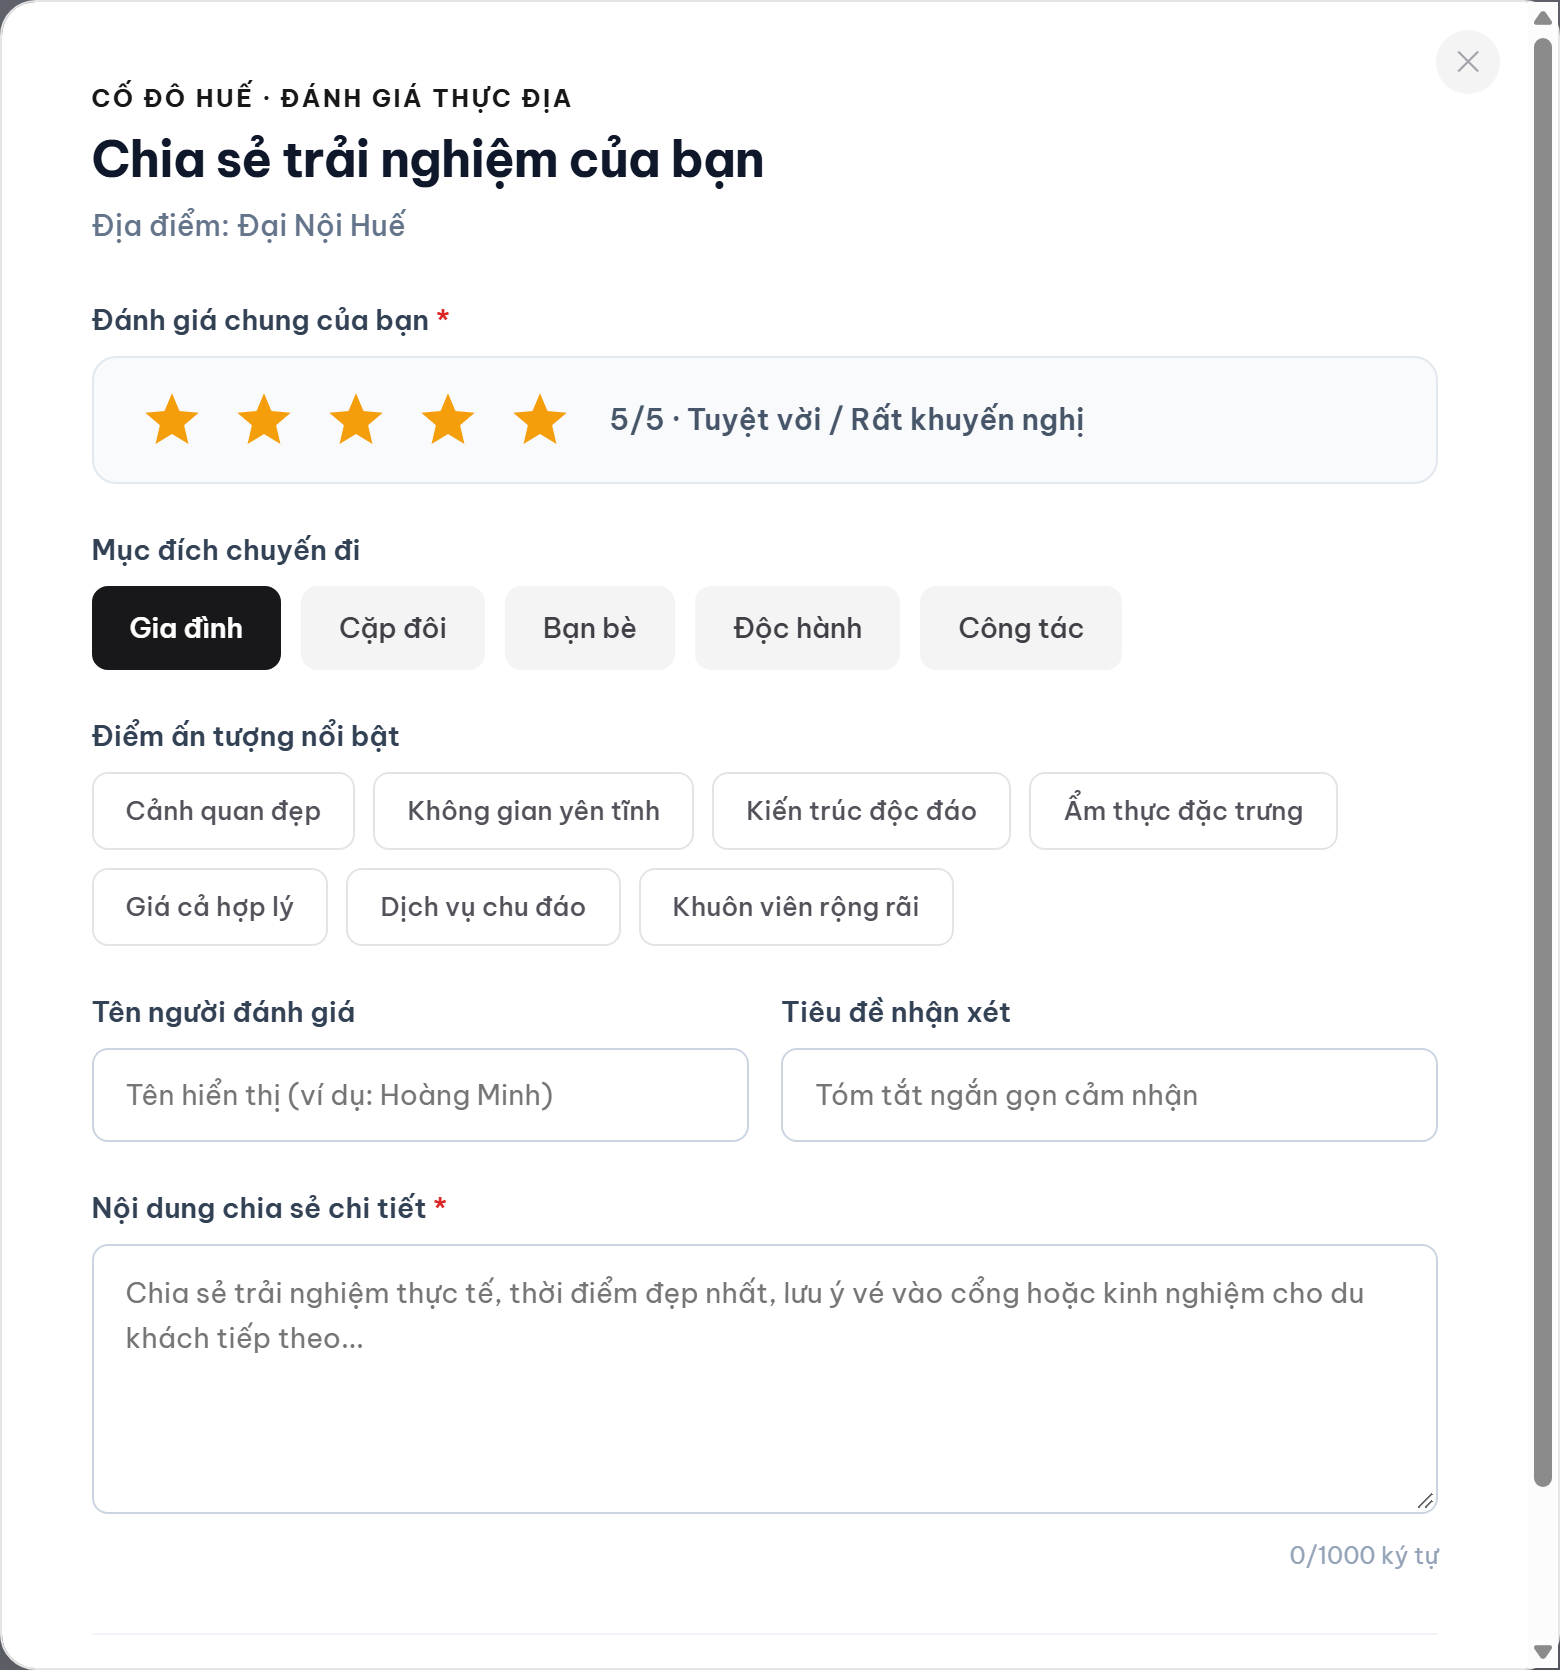
\includegraphics[width=0.58\textwidth]{img/web_poi_review_modal.png}
    \caption{Cửa sổ Gửi Đánh giá và Phản hồi Trải nghiệm Du khách Thực địa (POI Review Modal)}
    \label{fig:web_poi_review_modal}
\end{figure}
